\documentclass{beamer}

\title{The Effect of Rotation on Stratified Turbulence}
\author[Dante Buhl]{Dante Buhl\\{\scriptsize Advised by: Pascale Garaud, Hongyun Wang}}
\date{August 22, 2024}
\institute{UCSC Applied Mathematics}
\graphicspath{ {./images/} }
\usepackage{verbatim}
\usetheme{Dresden}
%\usecolortheme{spruce}
\usecolortheme{dolphin}
\usefonttheme{serif}
\usepackage{amsmath}
\usepackage{pifont}
\usepackage{hyperref}
\usepackage{amsthm} %proof environment
\usepackage{amssymb}
\usepackage{amsfonts}
%\usepackage{enumitem} %nice lists
\usepackage{verbatim} %useful for something 
\usepackage{xcolor}
\usepackage{blindtext} % I have no idea what this is 
\usepackage{caption}  % need this for unnumbered captions/figures
\usepackage{soul} % need this for the hl command
\usepackage{graphicx} % Required for inserting images
\usepackage{multimedia}
\usepackage{natbib}

\begin{document}

\newcommand{\wrms}{w_{\text{rms}}}
\newcommand{\bs}[1]{\boldsymbol{#1}}
\newcommand{\tb}[1]{\textbf{#1}}
\newcommand{\bmp}[1]{\begin{minipage}{#1\textwidth}}
\newcommand{\emp}{\end{minipage}}
\newcommand{\R}{\mathbb{R}}
\newcommand{\C}{\mathbb{C}}
\newcommand{\N}{\mathcal{N}}
\newcommand{\K}{\bs{\mathrm{K}}}
\newcommand{\m}{\bs{\mu}_*}
\newcommand{\s}{\bs{\Sigma}_*}
\newcommand{\dt}{\Delta t}
\newcommand{\dx}{\Delta x}
\newcommand{\tr}[1]{\text{Tr}(#1)}
\newcommand{\Tr}[1]{\text{Tr}(#1)}
\newcommand{\Div}{\nabla \cdot}
\renewcommand{\div}{\nabla \cdot}
\newcommand{\Curl}{\nabla \times}
\newcommand{\Grad}{\nabla}
\newcommand{\grad}{\nabla}
\newcommand{\grads}{\nabla_s}
\newcommand{\gradf}{\nabla_f}
\newcommand{\xs}{\bs{x}_s}
\newcommand{\xf}{\bs{x}_f}
\newcommand{\ts}{t_s}
\newcommand{\tf}{t_f}
\newcommand{\pt}{\partial t}
\newcommand{\pz}{\partial z}
\newcommand{\uvec}{\bs{u}}
\newcommand{\F}{\bs{F}}
\newcommand{\T}{\tilde{T}}
\newcommand{\ez}{\bs{e}_z}
\newcommand{\ex}{\bs{e}_x}
\newcommand{\ey}{\bs{e}_y}
\newcommand{\eo}{\bs{e}_{\bs{\Omega}}}
\newcommand{\ppt}[1]{\frac{\partial #1}{\partial t}}
\newcommand{\ppts}[1]{\frac{\partial #1}{\partial t_s}}
\newcommand{\pptf}[1]{\frac{\partial #1}{\partial t_f}}
\newcommand{\ppz}[1]{\frac{\partial #1}{\partial z}}
\newcommand{\ddz}[1]{\frac{d #1}{d z}}
\newcommand{\ppzetas}[1]{\frac{\partial^2 #1}{\partial \zeta^2}}
\newcommand{\ppzs}[1]{\frac{\partial #1}{\partial z_s}}
\newcommand{\ppzf}[1]{\frac{\partial #1}{\partial z_f}}
\newcommand{\ppx}[1]{\frac{\partial #1}{\partial x}}
\newcommand{\ppy}[1]{\frac{\partial #1}{\partial y}}
\newcommand{\ppzeta}[1]{\frac{\partial #1}{\partial \zeta}}


\begin{comment}
    1. Intro 
    2. Model
        - new forcing mechanism
    3. Previous Work?
        - Multiscale theory by Chini et al and Shahe et al
    4. Stochastically forced Stratified TurbulenceA
        - new horizontal structures in the flow
        - weak correlation between vertical vorticity and mixing
        - previous wmrs scalings aren't as effective
    5. Rotating Stratified Turbulence
        - new flow structures (columns appear in the flow)
        - mixinng is localized to anti-cyclones
        - inverse energy cascade to small horizontal wavenumbers
        - decline in vertical mixing 
        
\end{comment}

\frame{\titlepage}

\section{Introduction}


\begin{frame}{Motivation}
% why do we care about stratified turbulence, what work inspires this project
\begin{itemize}
\item  Stratified Turbulence is characterized by three-dimensional anisotopic turbulence where vertical motions are limited due to stratification. 

\item Many geophysical and astrophysical flows are stably stratified and rotating (e.g. oceans, atmosphere, stellar interiors, gas giants).

\item How much vertical mixing takes places in these flows? 

\item How does mixing depend on flow parameters?

%a terminology introduced by D. K. Lilly to describe flows that exhibit three-dimensional anisotropic turbulence where vertical motions are limited due to stratification \citep{Lilly1983}.
%Stratification is defined to be the presence of a stable density profile $\bar\rho(z)$ whereby the density increases with depth ($d\bar \rho/dz <0$). Displaced fluid parcels feel a restoring buoyancy force, which pulls them back toward equilibrium. The strength of the stratification is measured by its buoyancy frequency $N = \sqrt{-gd\ln(\bar{\rho})/dz}$ where $g$ is the local gravity. Many geophysical and astrophysical systems have stratified regions, including the Earth's oceans and atmosphere and the radiative zones of stars and planets. The source of the stratification can either be temperature or composition (e.g. salinity in the oceans, helium content in stars). 

\end{itemize}


\end{frame}

\begin{frame}{Schematic}
    \includegraphics[width = \textwidth]{files/PADDIM Schematic.pdf}

    %\hl{add temp profile, gravity}
    % Notes: Tripply Periodic Domain with dimensions 4pi x 4pi x pi. We notice
    % the rotation vector omega placed in the diagram to visualize the angle of
    % rotation with respect to gravity (or the vertical coordinate direction).
    % It should also be noted that the rotation vector should be pointing in the
    % y direction. 
    % For the results you will be seeing today, rotation has not yet been
    % included, but it is the next step for our parameter study. 
\end{frame}

\begin{frame}{Governing Equations}

    {\small
    \begin{align}
        \ppt{\bs{u}} + \uvec \cdot \Grad \uvec +
        \frac{1}{Ro}(\ez \times
        \uvec) &= -\Grad p +
        \frac{T}{Fr^2}\ez + \F + \frac{1}{Re}\Grad^2\uvec \tag{mom.}\label{eq:momentum}\\
        \ppt{T} + \bs{u} \cdot \Grad T + w &= \frac{1}{Pe}\Grad^2T \tag{temp.} \label{eq:temp} \\
        \Div \bs{u} &= 0 \tag{cont.}\label{eq:cont}
    \end{align}
    
    \begin{align*}
        Re = \frac{UL}{\nu}, \quad Pe = \frac{UL}{\kappa}, \quad Fr =
        \frac{U}{NL}, \quad Ro = \frac{U}{2\Omega L}
    \end{align*}
    }
    \begin{itemize}
        \item $U$ is the characteristic velocity
        \item $L$ is the large eddy horizontal length scale
        \item $N$ is the buoyancy frequency ($N = \sqrt{\alpha_Tg\ddz{\bar{T}}}$)
        \item $\Omega$ is the angular velocity
        \item $(\nu, \kappa)$ are the (viscous, thermal) diffusivity coefficients
    \end{itemize}
    %Where $U$ is the characteristic velocity, $L$ is the eddy length scale, $N$ is the buoyancy frequency, and $\Omega$ is the angular velocity of the rotating body. 
    % Notes: Classic Non-dimensionalized Boussinesue Rotations which include a
    % buopyancy field, viscous and dissipative dynamics, as well as rotation
    % (the coriolis force). Thus we see the appearnce of the Rossby, Froude,
    % Reynolds, and Peclet numbers in the governing equations. It should b
    % mentioned that this rotation vector r = <0, sin(\phi), cos(\phi)>. 

\end{frame}

\begin{frame}{Stratified Turbulence}

    \begin{itemize}
        \item Large scale flow is anisotropic.
        \item Small scale flow is isotropic.
    \end{itemize}

\begin{center}
    \includegraphics[width=\textwidth]{files/StratifiedTurbulence.png}
\end{center}
\end{frame}

\begin{frame}{Multiscale Theory \citep{Chinial2022}}

    Schematic model for stratified turbulence:
    \begin{center}
    \includegraphics[width=1\textwidth]{files/Multi-Scale Schematic.pdf}
    \end{center}
    \vspace{20pt}
    \citet{Chinial2022} developed a multiscale theory dependent on the aspect ratio $\alpha = l_z/L \ll 1$ where $l_z$ is the vertical length scale of the eddies. 

    % notes: - mean flow describes the large-scale eddies, 
    %        - fluctuations describe the small-scale eddies
    
\end{frame}

\begin{frame}{Multiscale Theory \citep{Chinial2022}}
    %Predicted Scaling laws

    \begin{itemize}
    \item Large scale, slow variables: $\xs = \bs{x}_h$, $\ts = t$
    \item Small scale, fast variables: $\xf = \bs{x}_h/\alpha$, $\zeta = z/\alpha$, $\tf = t/\alpha$.
    \item Each variable $q = q(\xs, \xf, \zeta, \ts, \tf)$
    \item Rescaled derivatives: $\grad_h = \grads + \alpha^{-1}\gradf$, $\ppz{} = \alpha^{-1}\ppzeta{}$, $\ppt{} = \ppts{} + \alpha^{-1}\pptf{}$
    \end{itemize}
    \vspace{10pt}
    Fast averaging is used to isolate ``mean'' ($\bar{q}(\xs, \zeta, \ts)$) and ``fluctuation'' ($q'(\xs,\xf,\zeta,\ts,\tf)$) dynamics
    \begin{gather*}
        q = \bar{q} + q', \quad \overline{q'} = 0
    \end{gather*}
\end{frame}

\begin{frame}{Multiscale Theory \citep{Chinial2022}}
    The governing equations are expanded:
    {\scriptsize
    \begin{align*}
        \eqref{eq:cont} \to \grads \cdot \bar{\uvec}_h + \frac{1}{\alpha} \ppzeta{\bar{w}} &= 0, \quad \bar{w} = O(\alpha)\\
        \frac{1}{\alpha}\gradf \cdot \uvec_h' + \frac{1}{\alpha} \ppzeta{w'} &= 0, \quad \uvec_h' = O(w')
    \end{align*}
    \begin{gather*}
        \eqref{eq:momentum}_h \downarrow\\
    \ppts{\bar{\uvec}_h} + \bar{\uvec}_h\cdot \grads\bar{\uvec}_h
    + \frac{1}{\alpha}\overline{\uvec_h'\cdot\gradf\uvec_h'}
    + \frac{\bar{w}}{\alpha}\ppzeta{\bar{\uvec}_h} 
    + \overline{\frac{w'}{\alpha}\ppzeta{\uvec_h'}}
    = -\grads\bar{p} + \bar{\F}_h + \frac{1}{\alpha^2Re}\ppzetas{\bar{\uvec}_h},\label{eq:horiz_mom_mean} \\
    \frac{1}{\alpha}\pptf{\uvec_h'} 
    + \frac{1}{\alpha}\bar{\uvec}_h\cdot\gradf\uvec_h'
    + \frac{w'}{\alpha}\ppzeta{\bar{\uvec}_h} 
    = -\frac{1}{\alpha}\gradf p' + \frac{1}{\alpha^2Re}\left( \gradf^2\uvec_h' + \ppzetas{\uvec_h'}\right), \label{eq:horiz_mom_perturbation}\\
    \to \uvec_h' = O(w') = O(\alpha^{1/2})
    \end{gather*}
    }
\end{frame}

\begin{frame}{Predicted Scaling Laws}

%The multiscale theory shows that mean vertical velocity scales as $\alpha$, and fluctuations to velocity scale as $\alpha^{1/2}$. The scaling of the temperature is dependent on the scaling of $Fr$ and $Pe$.
Using the multiscale theory to investigate the vertical momentum and temperature equations reveals that there are two regimes of stratified turbulence ($Fr \ll 1$). 

\vspace{10pt} 

\begin{itemize}
\item Non-diffusive ($Fr^2Pe \ge O(1)$) \citep{Chinial2022}: $\alpha = Fr$
\item Thermally diffusive ($Fr^2Pe \ll O(1)$) \citep{Shah2023}: $\alpha = (Fr^2/Pe)^{1/3}$
\end{itemize}

In this thesis, we focus on the non-diffusive case.
\end{frame}

\begin{frame}{Scaling Law Validation}
    % wrms plot and lz plot
    Direct numerical simulations validated the scaling laws derived from the multiscale theory. 

    \bmp{.29}
        {\small
        {\color{blue}
        \[
            w_{turb} =
            \sqrt{\frac{\left<w^2\omega_z^2\right>}{\left<\omega_z^2\right>}}
        \]
        }{\color{red}
        \[
            w_{lam} =
            \sqrt{\frac{\left<w^2\omega_z^{-2}\right>}{\left<\omega_z^{-2}\right>}}
        \]
        }}
    \emp
    \bmp{.7}
        \centering
        \includegraphics[width=\textwidth]{files/Garaudwrms.png}
    \emp
    
\end{frame}


\section{Stochastic Forcing}

% why do we run these DNS
\begin{frame}{Why use stochastic forcing?}

    \begin{itemize}
    \item Previous studies \citep{Copeal2020,Garaud2020,Garaudal2024} have used steady forcing in direct numerical simulations.
    \item Steady forcing is inadequate in the rapidly rotating limit.%We avoid steady forcing so that the Coriolis force cannot produce unrealistic, stable span-wise flows.
    \item Stochastic forcing has been used in several prior studies \citep{HerringMetais1989,WaiteBartello2004,WaiteBartello2006,Lindbord2006,Maffioli_Brethouwer_Lindborg_2016,Waite2017}. 
    \end{itemize}

\end{frame}

\begin{frame}{Forcing Mechanism}

    We choose our forcing to be purely horizontal and divergence-free:
    \[
        \bs{F} = F_x\ex + F_y\ey, \quad \grad \cdot \uvec = 0
    \]
    The forcing is applied in spectral space and satisfies $\bs{k} \cdot \hat{\bs{F}} = 0$:
    \begin{gather*}
        \hat{F}_x = \frac{k_y}{|\bs{k}_h|}G(\bs{k}_h,t), \quad \hat{F}_y = \frac{-k_x}{|\bs{k}_h|}G(\bs{k}_h,t)\\
        G(\bs{k}_h,t) \in \C
    \end{gather*}
    where $G(\bs{k}_h,t)$ is a Gaussian process of amplitude 1 and correlation timescale 1. 

\end{frame}

% what changes about the forcing
\begin{frame}{Gaussian processes as a stochastic method}
    %We use Gaussian processes in order to generate stochastic forcing. 
    \begin{itemize}
        \item Generates points according to prescribed mean and covariance functions.
        \item Easy parameterization of forcing properties.
    \end{itemize}

    \bmp{1}
        \centering
        \bmp{.2}
            \raggedleft {\scriptsize $G(t)$}
        \emp
        \bmp{.55}
        \includegraphics[width=1\textwidth]{files/forcing_example.pdf}
        \emp
        \bmp{.2}
        {\color{white} shdjajkd}
        \emp
    \emp
    
\end{frame}



% what are the flow structures that we obtain?
\begin{frame}{Flow Structure}
    % Ux rms figure
    % plot info: B100 is -3.5:3.5
    % B300 is -5:5
    % B10 is -3:3
    %B1 is -5:5
    \centering
    \bmp{.235}
        \centering
        $1/Fr = 1$
        \vspace{2pt}
        
        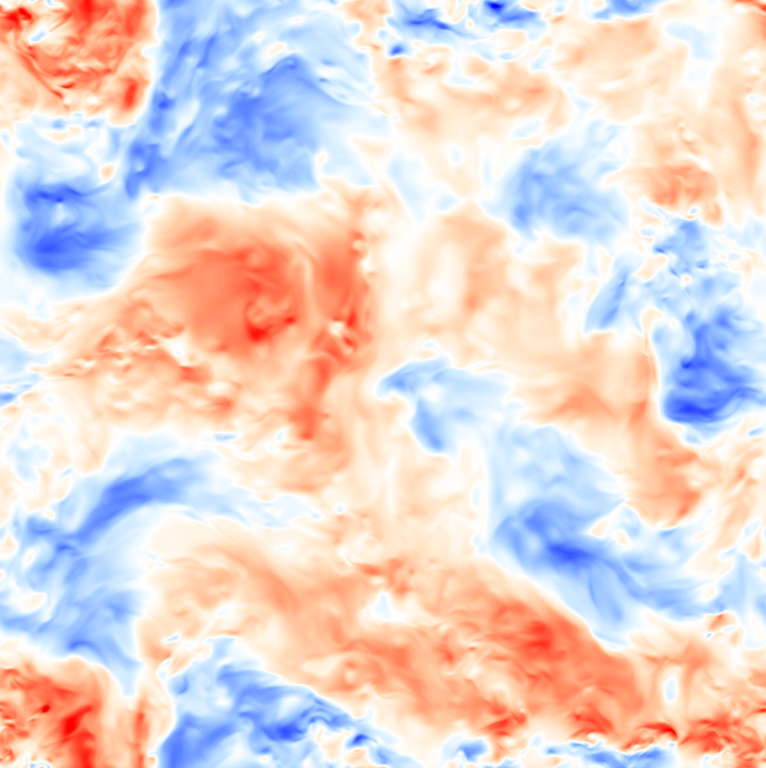
\includegraphics[width=\textwidth]{files/XYB1ux.png}
        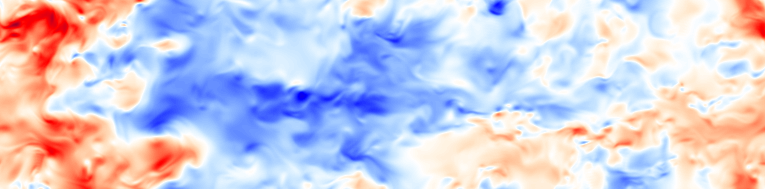
\includegraphics[width=\textwidth]{files/XZB1ux.png}
        \includegraphics[width = \textwidth]{files/B1Spec.pdf}
    \emp
    \hspace{1pt}
    \bmp{.235}
        \centering
        $1/Fr = 3.16$
        \vspace{2pt}
        
        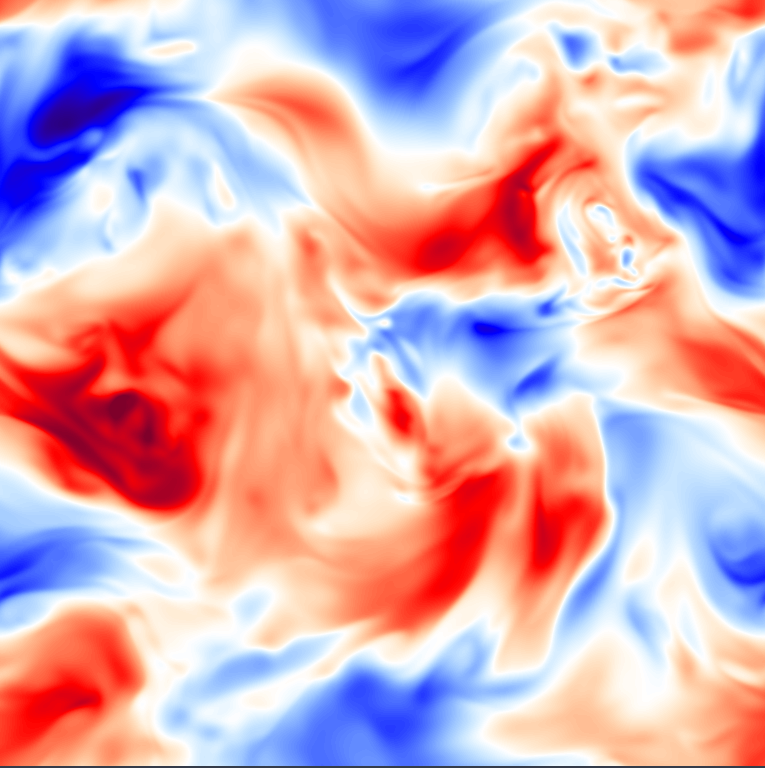
\includegraphics[width=\textwidth]{files/XYB10ux.png}
        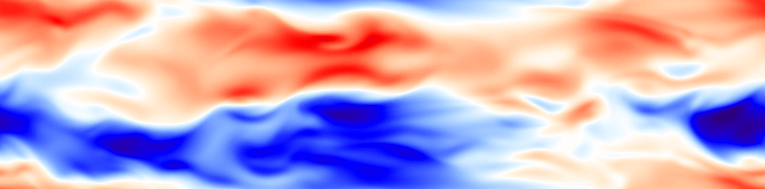
\includegraphics[width=\textwidth]{files/XZB10ux.png}
        \includegraphics[width = \textwidth]{files/B10Spec.pdf}
    \emp
    \hspace{1pt}
    \bmp{.235}
        \centering
        $1/Fr = 10$
        \vspace{2pt}
        
        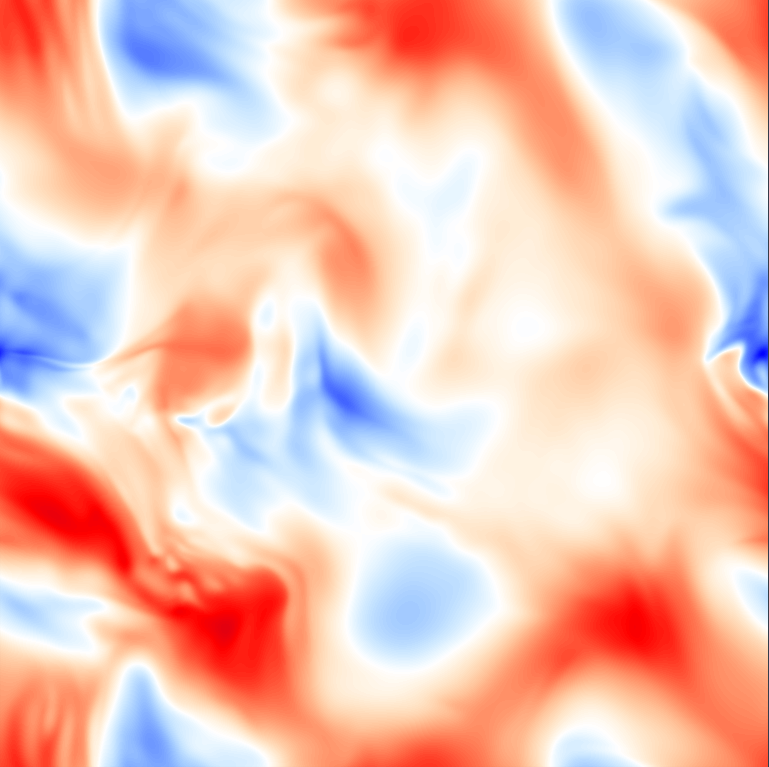
\includegraphics[width=\textwidth]{files/XYB100ux.png}
        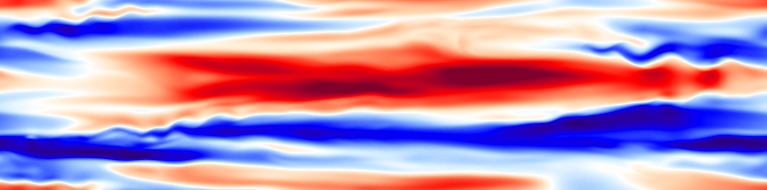
\includegraphics[width=\textwidth]{files/XZB100ux.png}
        \includegraphics[width = \textwidth]{files/B100Spec.pdf}
    \emp
    \hspace{1pt}
    \bmp{.235}
        \centering
        $1/Fr = 17.36$
        \vspace{2pt}
        
        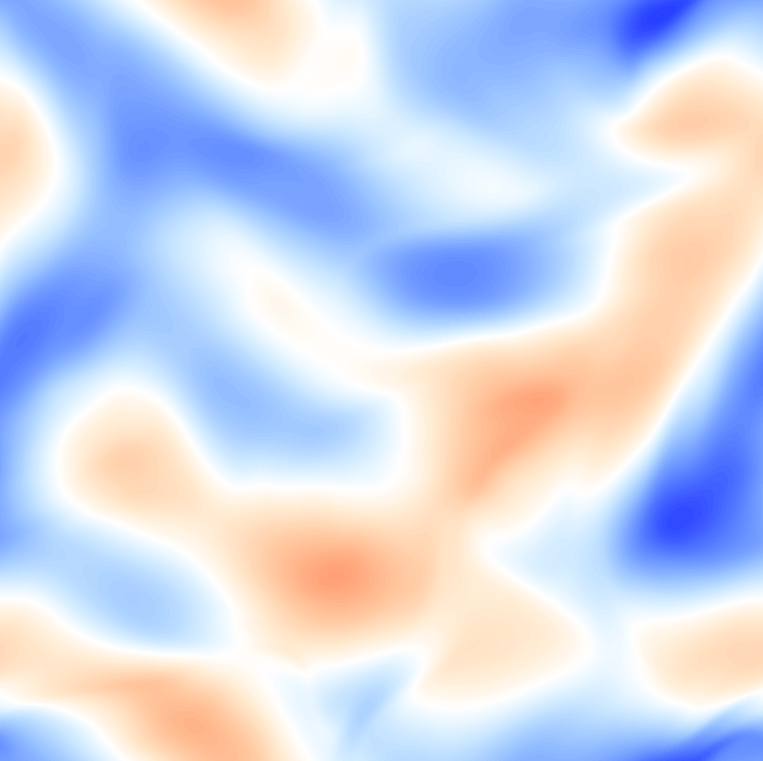
\includegraphics[width=.99\textwidth]{files/XYB300ux.png}
        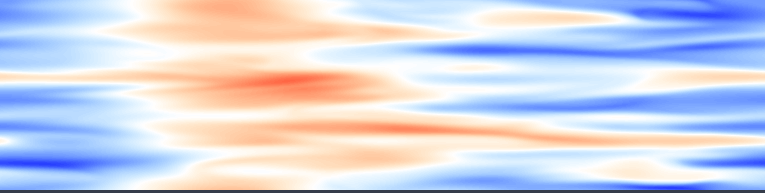
\includegraphics[width=.99\textwidth]{files/XZB300ux.png}
        \includegraphics[width = \textwidth]{files/B300Spec.pdf}
    \emp
    \[\overrightarrow{\rm Stratification}\]
\end{frame}

\begin{comment}
\begin{frame}{Energy Spectrum}
    \centering
    \begin{figure}
        \small
        \bmp{0.235}
            \centering
            \subcaption{$1/Fr$ = 1}
        \emp
        \bmp{0.235}
            \centering
            \subcaption{$1/Fr$ = 3.16}
        \emp
        \bmp{0.235}
            \centering
            \subcaption{$1/Fr$ = 10}
        \emp
        \bmp{0.235}
            %\subcaption{$Fr^{-2}$ = 100}
            \centering
            \subcaption{$1/Fr$ = 17.32}
        \emp
        \normalsize
        % Notes: We see the higher Froude Numbers follow the kolmogorov scaling
        % of k**(-5/3) after the flow becomes isotropic. While the flow is
        % anisotropic it follows the k**-3 scaling well except for K<1 for some
        % reason (more to investigate about this later). The energy spectrum
        % lacking the kolmogorov dissipative scaling suggests that the flow is
        % sufficiently turbulent at higher B values. This suggests that the
        % difference in the energy inhection scale might be lowereing the
        % effective reynolds number. 
    \end{figure}
\end{frame}
\end{comment}


% how does this affect mixing and turbulence
\begin{frame}{Weighted $w_{rms}$ scaling}
    \centering 
    \bmp{.29}
        {\small
        {\color{blue}
        \[
            w_{turb} =
            \sqrt{\frac{\left<w^2\omega_z^2\right>}{\left<\omega_z^2\right>}}
        \]
        }{\color{red}
        \[
            w_{lam} =
            \sqrt{\frac{\left<w^2\omega_z^{-2}\right>}{\left<\omega_z^{-2}\right>}}
        \]
        }}
    \emp
    \bmp{.7}
        \centering
        \includegraphics[width =\textwidth]{files/wrms_plot_nonrotating.pdf}
        \includegraphics[width =\textwidth]{files/wrms_key_slides.pdf}
    \emp
    % Notes: This scaling doesn't match the previous findings perfectly. As was
    % noted in pervious papers, we expected the turbulent w_rms to scale by
    % Froude to the 1/2, and the laminar w_rms to scale with Froude. As seen
    % here however, the predicted scaling do not seem to appear here. More
    % importantly, the turbulent and laminar w_rms both seem to follow the same
    % scaling, that is they do not diverge from each other as seen in previous
    % results. 
    % Note: W_turb arises from the multiscale analysis and when non-diffusive should scale with
    % froude to the half (source: Brethower et al (2007), Billant and Chomex (2001))
    % W_lam is recovered with the single scale analysis and when non-diffusive should scale with
    % froude (source: Chini et al. (2022), Riley and Lindbord (2012))
    % Explain the weighed wrms definitions.
\end{frame}


\begin{frame}{Mixing Efficiency, $\eta$}
    \centering

    \bmp{.3}
        \begin{gather*}
            \eta = \frac{\chi}{\chi + \epsilon}\\
            \chi = \frac{\left<|\grad T|^2\right>}{Fr^2Pe}\\
            \epsilon = \frac{\left<|\grad \uvec|^2\right>}{Re}
        \end{gather*}
    \emp
    \bmp{.7}
        \includegraphics[width = \textwidth]{files/mixing_plot_nonrotating.pdf}
    \emp
    % Notes: Here is the plot of the mixing efficiency as a function of the B
    % value (froude **-.5). We can see that this suggests that the effective
    % froude number might be different from that of simulations with the
    % sinusoidal shear forcing. It seems that the plateau of the mixing
    % efficiecy starts at lower B values in previous simualtions than in the
    % results shown here. 
\end{frame}

\begin{comment}
\begin{frame}{Discussion}

    \begin{itemize}
        \item What might be ideal parameters to directly compare new simulations
        to previous?
        \item Are the weighted $w_{rms}$ definitions still valid in a
        multi-directionally forced flow? 
        % sin shear flows seemed successful with weighted w values. In a flow
        % forced in x and y, is the vertical vorticity still a valid model (will
        % it pick up intermediate eddy scales?)
        % Is there a differnt multiscale analysis that we can expect with such a
        % forcing?
    \end{itemize}

\end{frame}
\end{comment}

\begin{comment}
\begin{frame}{Mixing and Vertical Vorticity }

    \bmp{0.49}
        \centering
        \includegraphics[width=1\textwidth]{files/vortz_pB400_vr.png}
    \emp
    \bmp{0.49}
        \centering
        \includegraphics[width=1\textwidth]{files/chi_pB400_vr.png}
    \emp
    
\end{frame}

\begin{frame}{Mixing and Vertical Vorticity}
    \centering
    \bmp{0.49}
        \centering
        \includegraphics[width=1\textwidth]{files/vortz_B180_vr2.png}
    \emp
    \bmp{0.49}
        \centering
        \includegraphics[width=1\textwidth]{files/chi_B180_vr2.png}
    \emp
\end{frame}
\end{comment}

\begin{frame}{Mixing and Vertical Vorticity }

    \bmp{.3}
        {\footnotesize\citep{Garaudal2024}}

        \vspace{100pt}

        {\footnotesize Stochastic DNS}
    \emp
    \bmp{0.35}
        \centering
        $\omega_z$
        \includegraphics[width=.9\textwidth]{files/vortz_pB400_vr.png}
        
        \includegraphics[width=.9\textwidth]{files/vortz_B180_vr2.png}
    \emp
    \bmp{0.35}
        \centering
        $|\grad T|^2/Pe$
        \includegraphics[width=.9\textwidth]{files/chi_pB400_vr.png}
        
        \includegraphics[width=.9\textwidth]{files/chi_B180_vr2.png}
    \emp
    
\end{frame}

\section{Rotation}

%set up
\begin{frame}{Rotating DNS}

We studied the effect of rotation by running two series of DNS, each set with a fixed Froude number and varying Rossby number. 
    
\end{frame}

%Numerical Restrictions
\begin{frame}{Numerical Constraints}
    \begin{itemize}
        \item The Courant condition limits the timestep of our DNS ($\dt \le \dx/|U|_{\rm max}$)
        \item Rapidly rotating DNS require smaller timesteps due to the amplitude of the horizontal velocity. 
    \end{itemize}
\end{frame}
 


\begin{frame}{Columnar Structures}
    \centering
    \bmp{.235}
        \centering
        $1/Ro = 0.5$
        \vspace{2pt}
        
        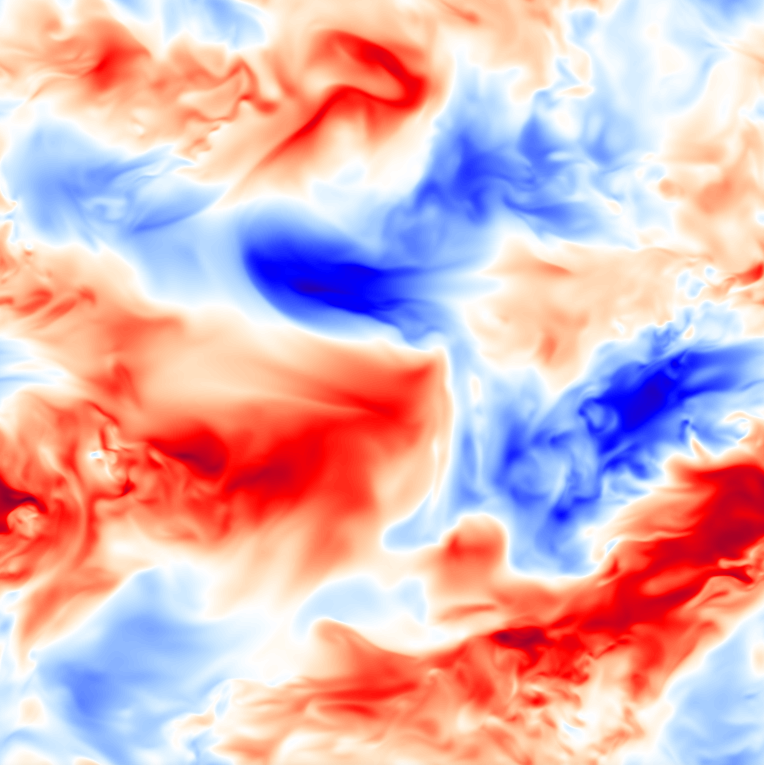
\includegraphics[width=\textwidth]{files/XYOm0.5ux.png}
        \includegraphics[width=\textwidth]{files/XZOm0.5ux.png}
    \emp
    \hspace{1pt}
    \bmp{.235}
        \centering
        $1/Ro = 1$
        \vspace{2pt}
 
        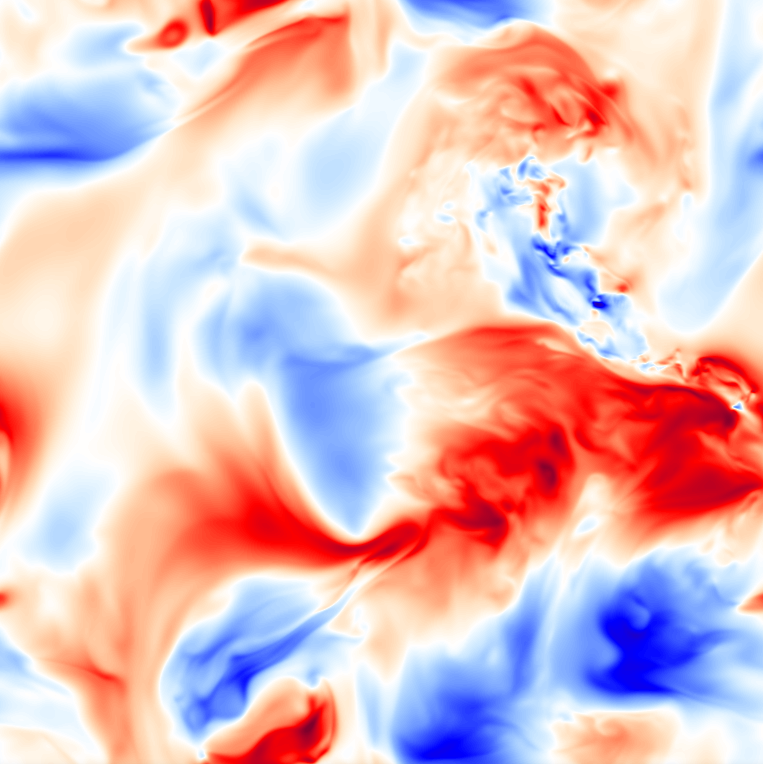
\includegraphics[width=\textwidth]{files/XYOm1ux.png}
        \includegraphics[width=\textwidth]{files/XZOm1ux.png}
    \emp
    \hspace{1pt}
    \bmp{.235}
        \centering
        $1/Ro = 2$
        \vspace{2pt}
        
        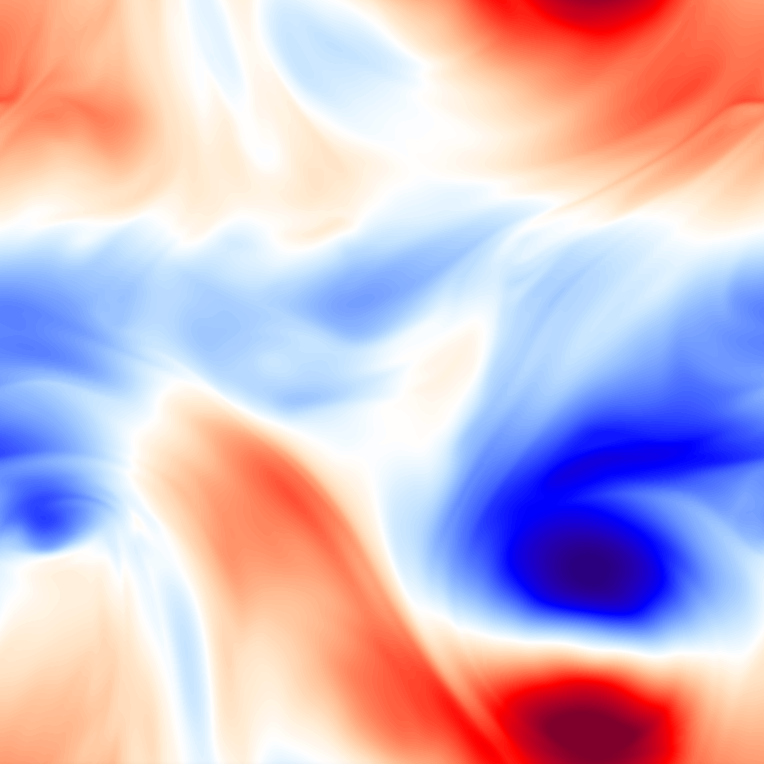
\includegraphics[width=\textwidth]{files/XYOm2ux.png}
        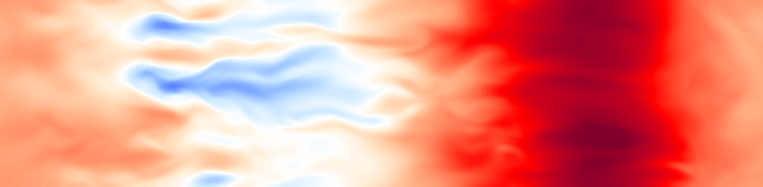
\includegraphics[width=\textwidth]{files/XZOm2ux.png}
    \emp
    \hspace{1pt}
    \bmp{.235}
        \centering
         $1/Ro = 4$
        \vspace{2pt}

        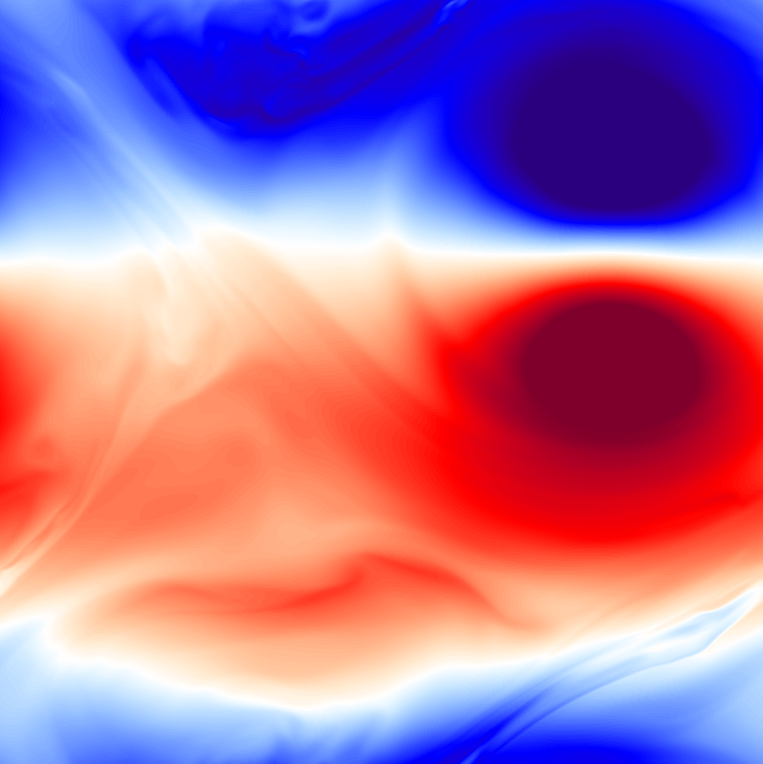
\includegraphics[width=\textwidth]{files/XYOm4ux.png}
        \includegraphics[width=\textwidth]{files/XZOm4ux.png}
    \emp
    \[\overrightarrow{\rm Rotation}\]
\end{frame}

\begin{frame}{Inverse Energy Cascade}
    \bmp{.33}
        \centering
        $Ro^{-1} = 0.5$
        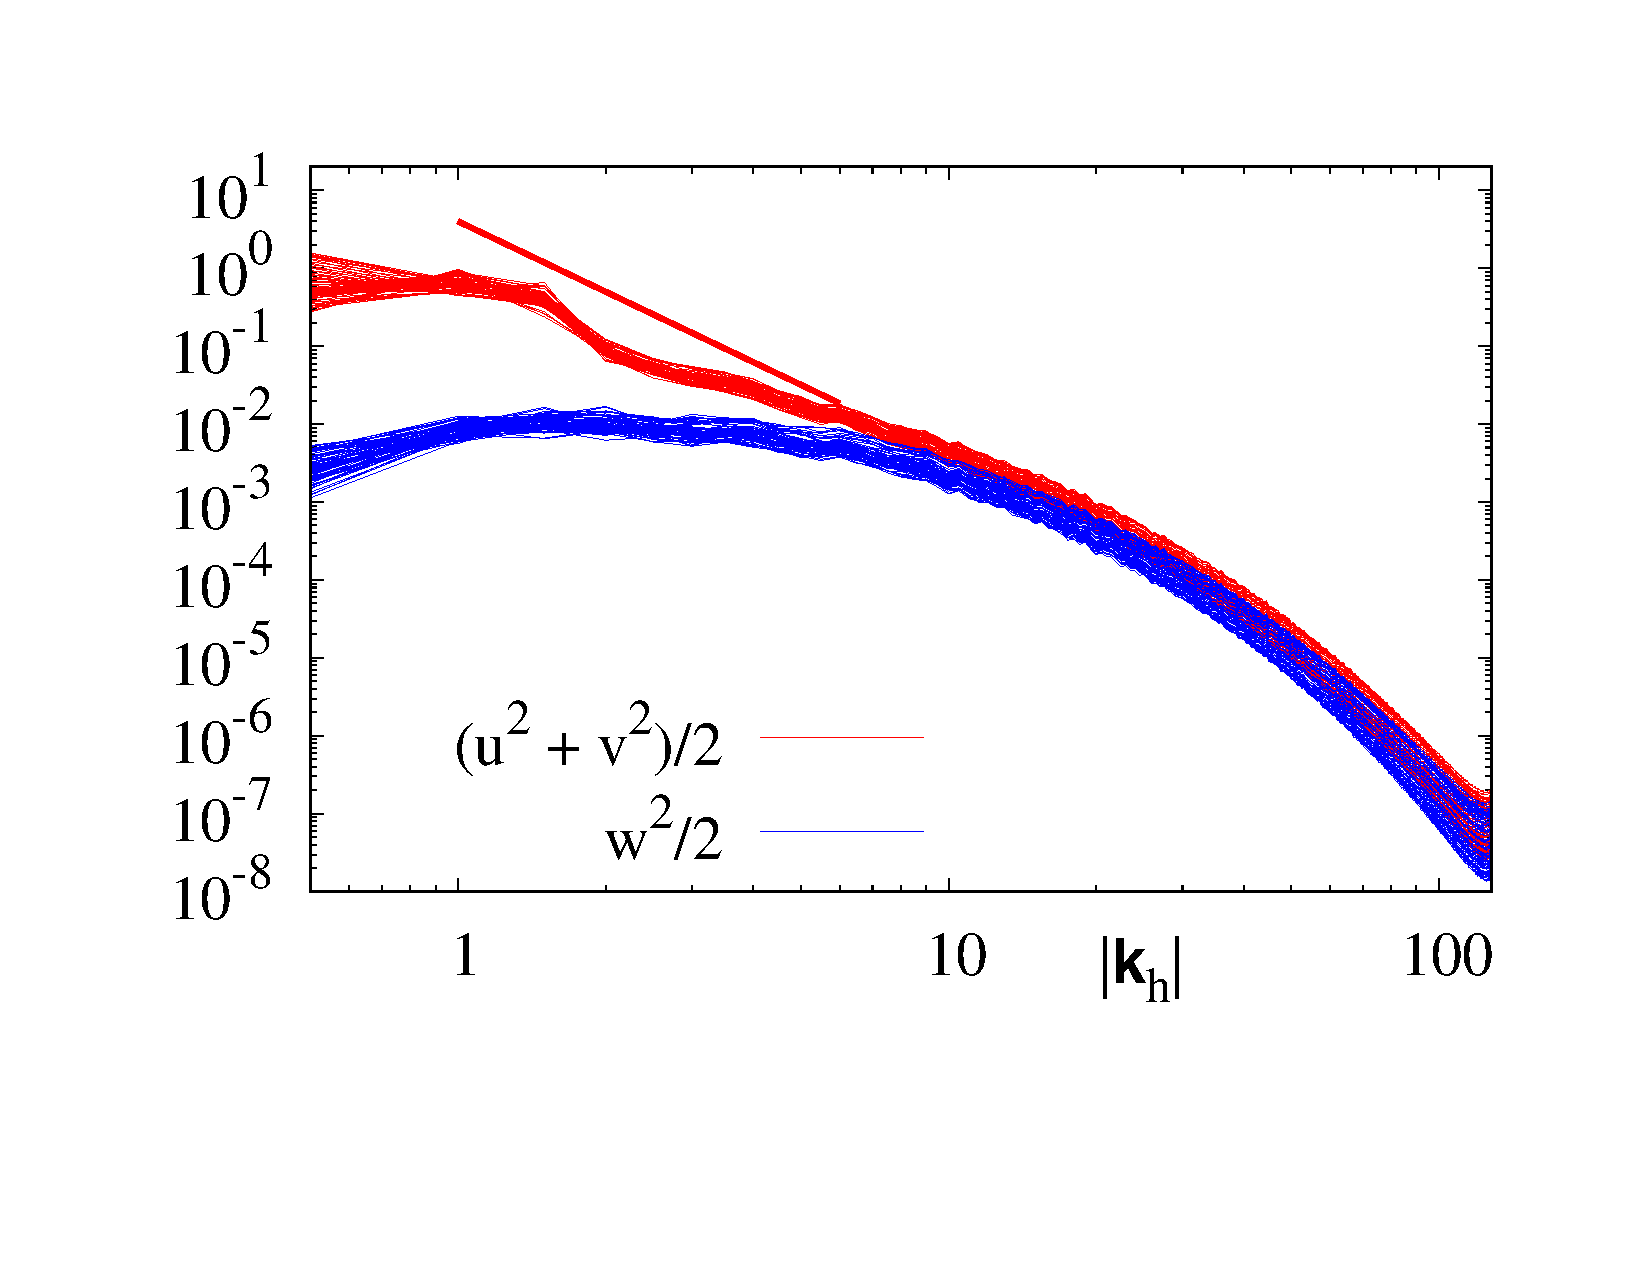
\includegraphics[width=.985\textwidth]{files/Om0.5Spec.pdf}
    \emp
    \bmp{.33}
        \centering
        $Ro^{-1} = 1$
        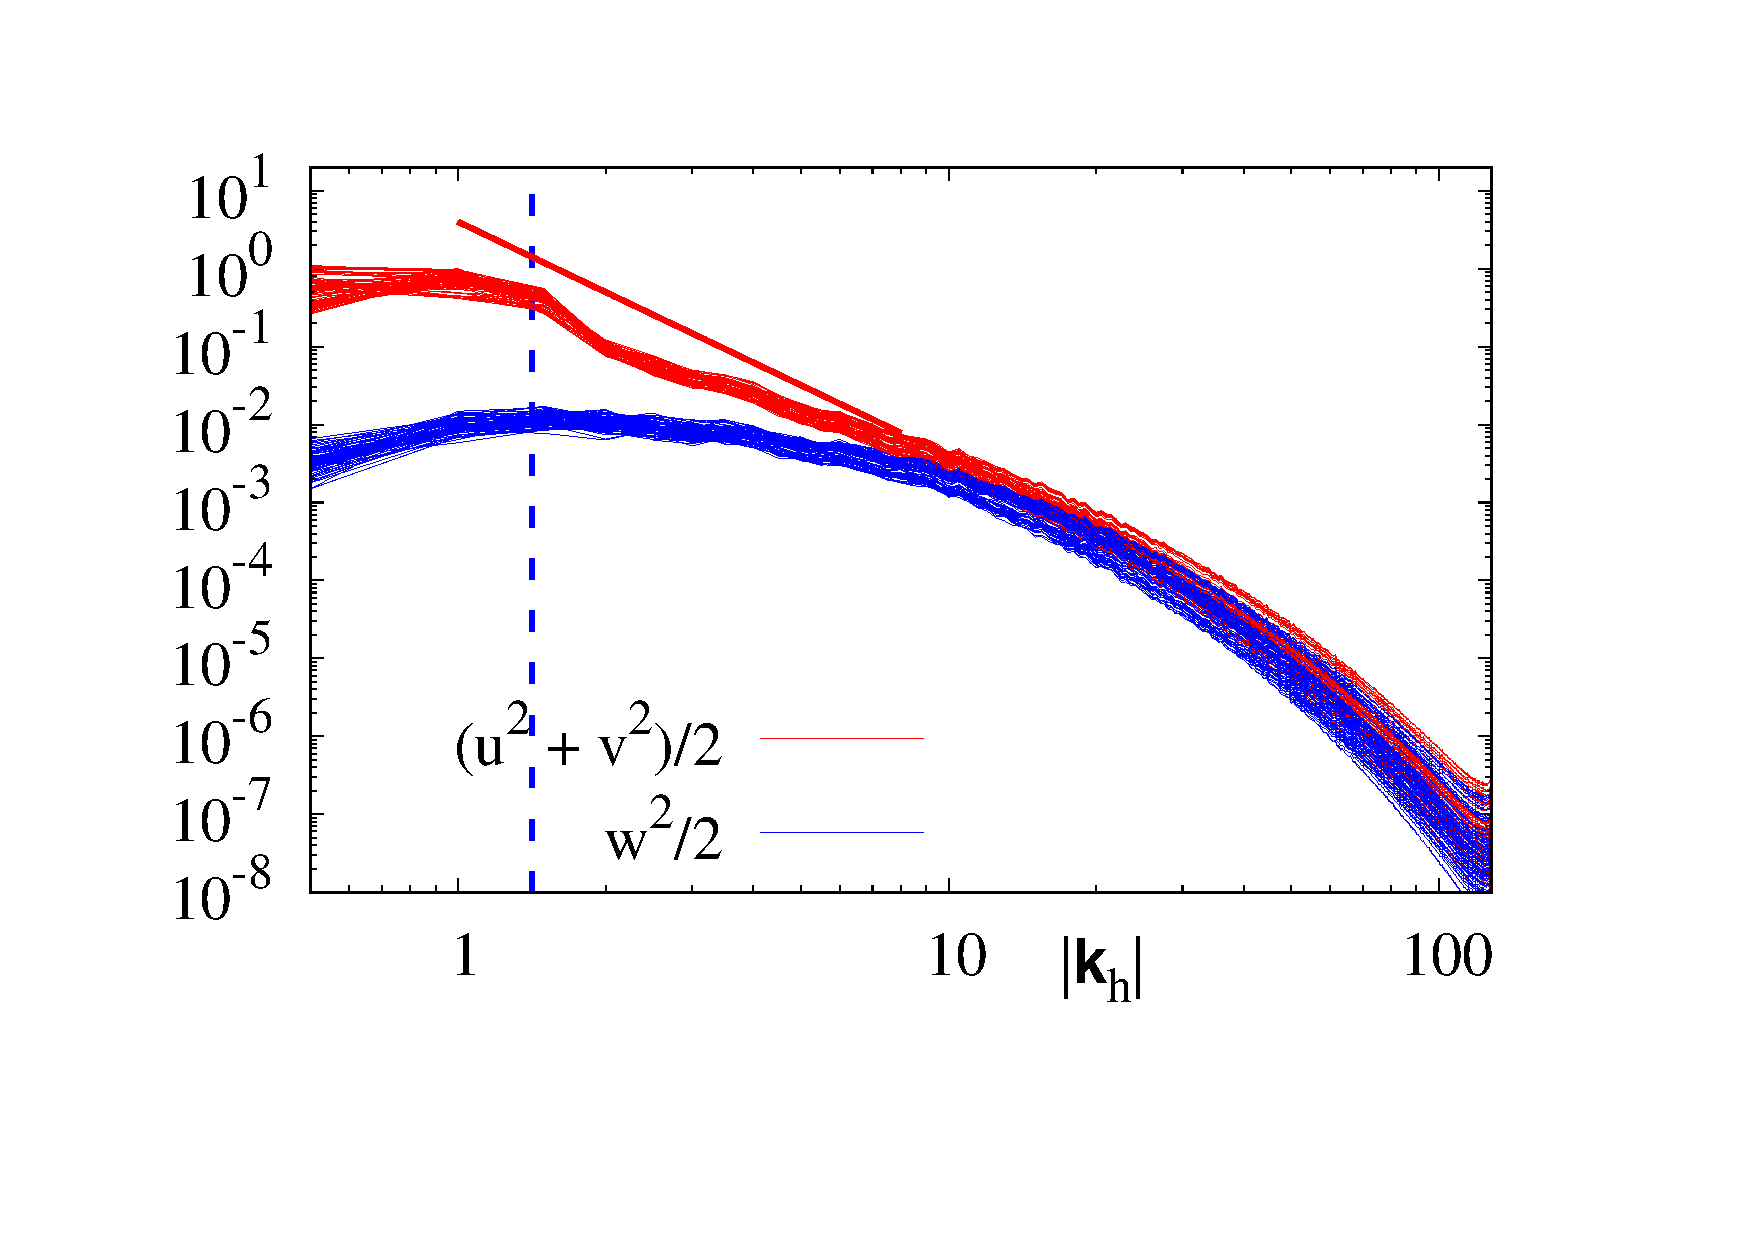
\includegraphics[width=\textwidth]{files/Om1Spec.pdf}
    \emp
    \bmp{.33}
        \centering
        $Ro^{-1} = 2$
        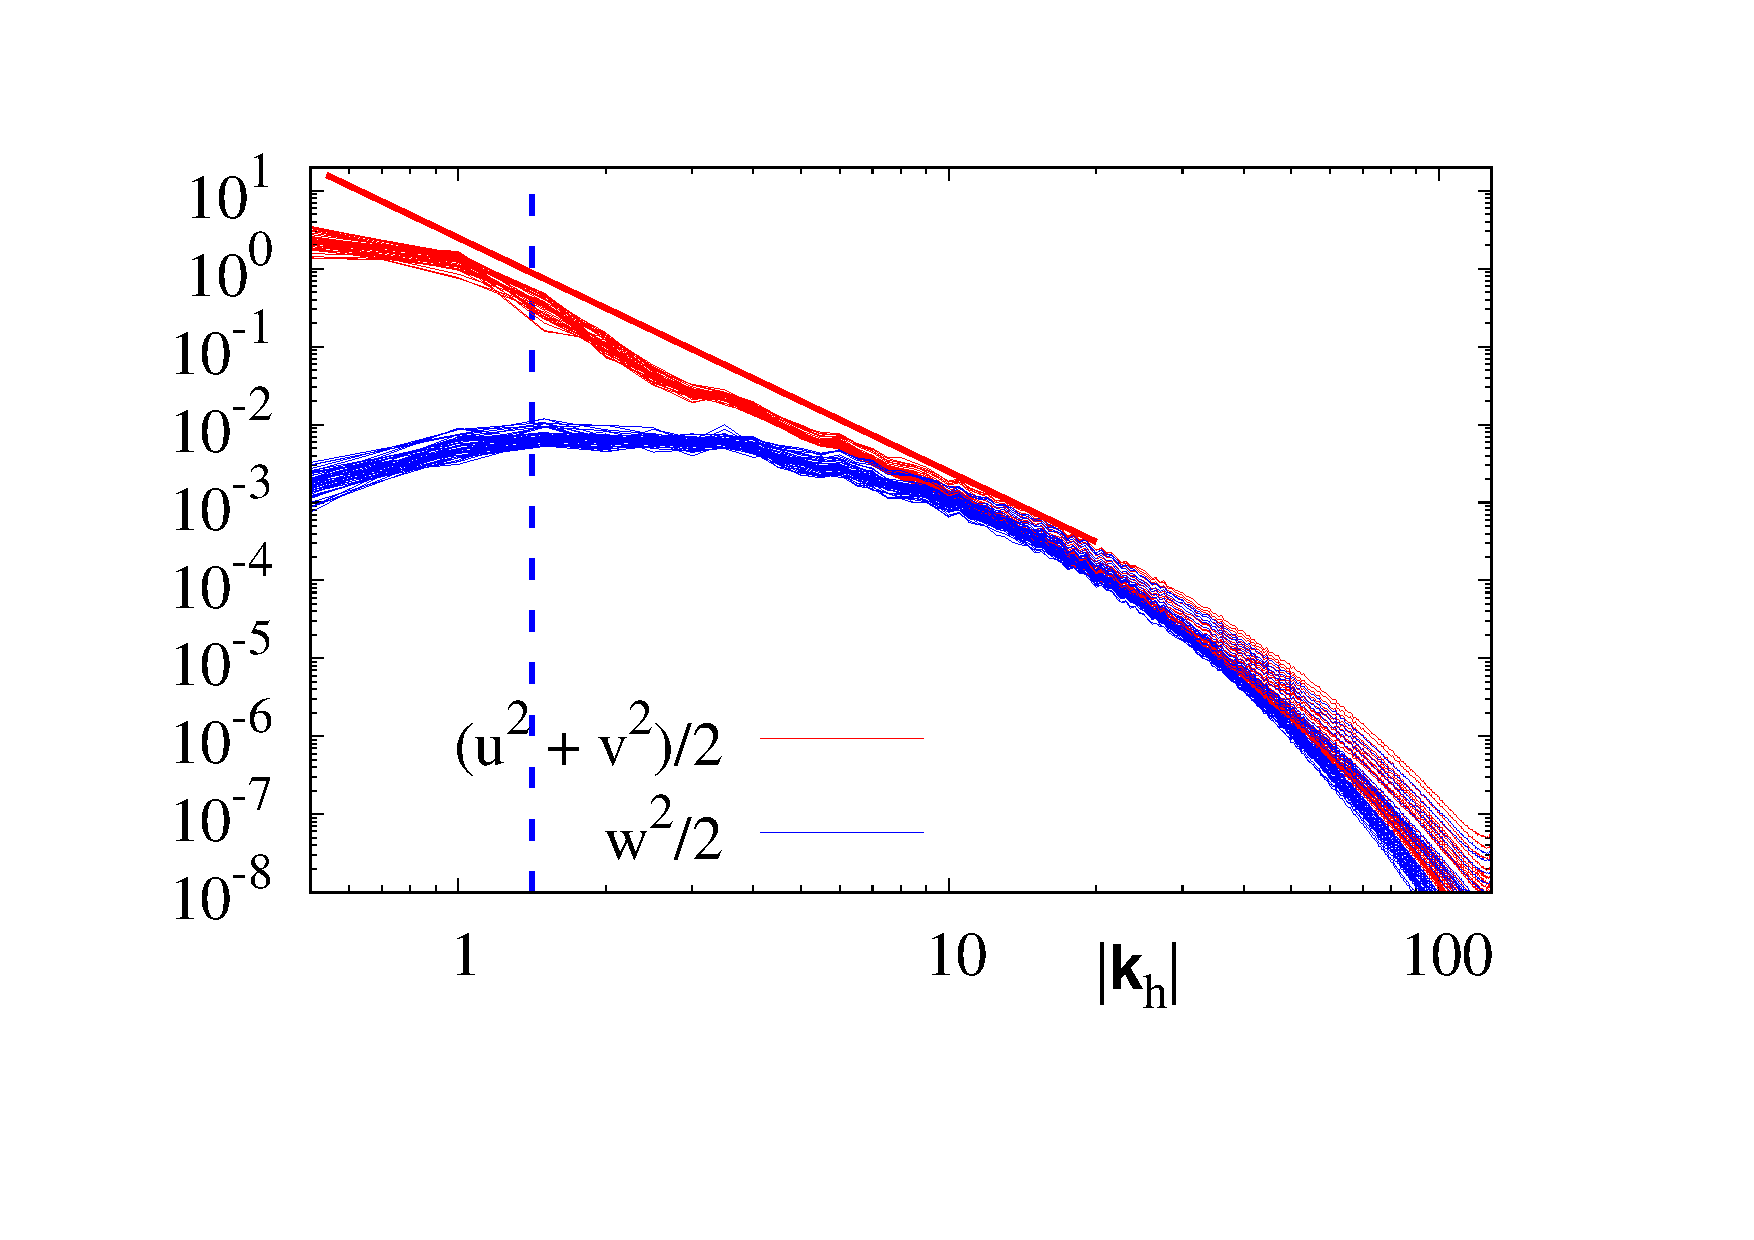
\includegraphics[width=1\textwidth]{files/Om2Spec.pdf}
    \emp
    
    \bmp{.33}
        \centering
        $Ro^{-1} = 4$
        \includegraphics[width=\textwidth]{files/Om4Spec.pdf}
    \emp
    \bmp{.33}
        \centering
        $Ro^{-1} = 5$
        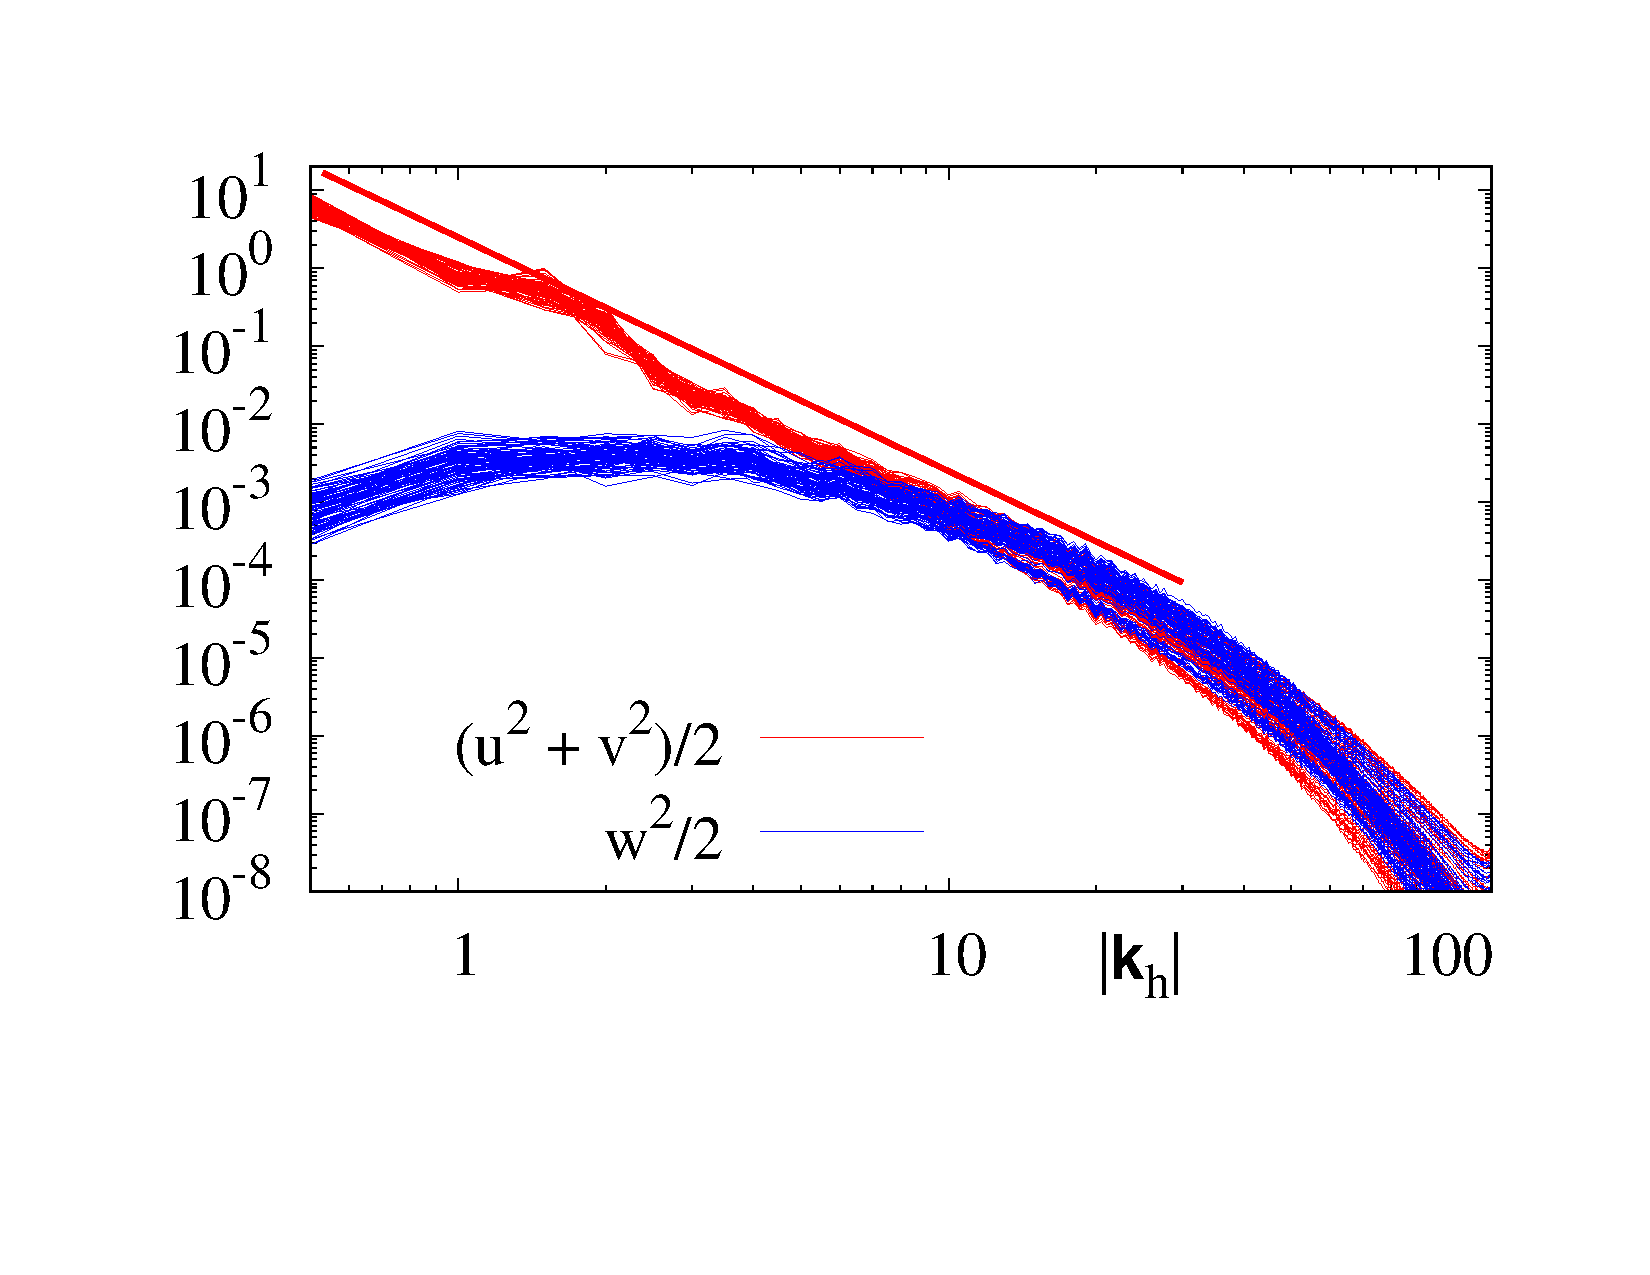
\includegraphics[width=1\textwidth]{files/Om5Spec.pdf}
    \emp
    \bmp{.33}
        \centering
        $Ro^{-1} = 10$
        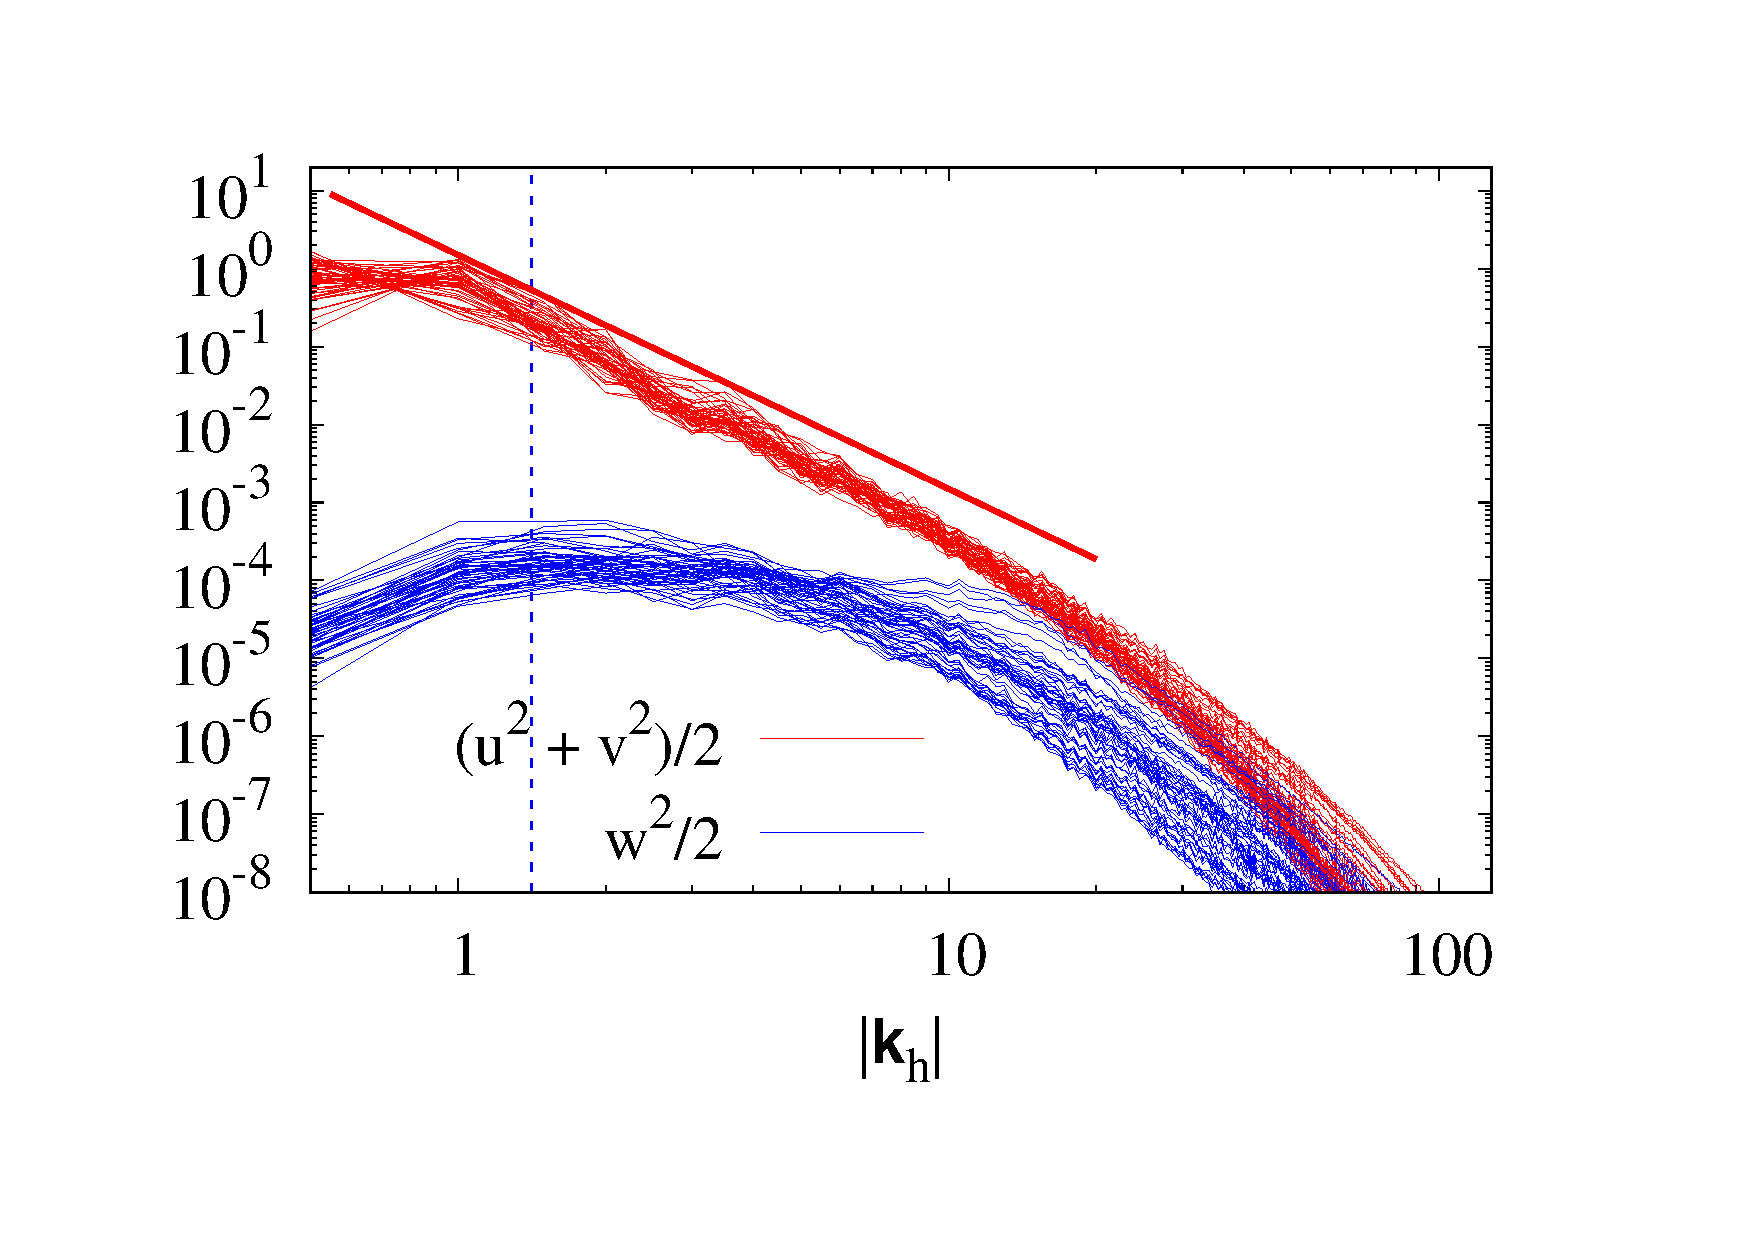
\includegraphics[width=\textwidth]{files/Om10Spec.pdf}
    \emp

\end{frame}

\begin{frame}{Mixing in the Flow}
    \bmp{0.07}
        $\omega_z$
        
        \vspace{75pt}
        
        $\frac{|\grad T|^2}{Pe}$
    \emp
    \bmp{.31}
        %omega_z
        \centering
        $1/Ro = 0.5$
        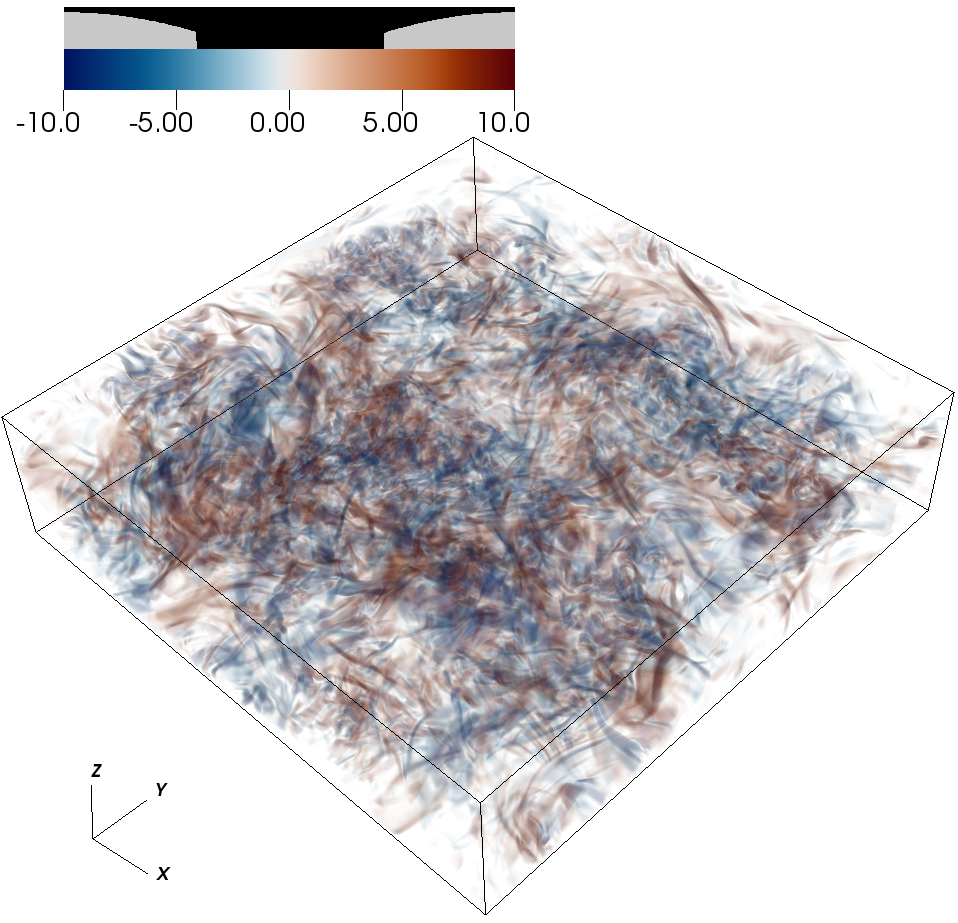
\includegraphics[width=.95\textwidth]{files/vortz_Om0.5_vr2.png}
        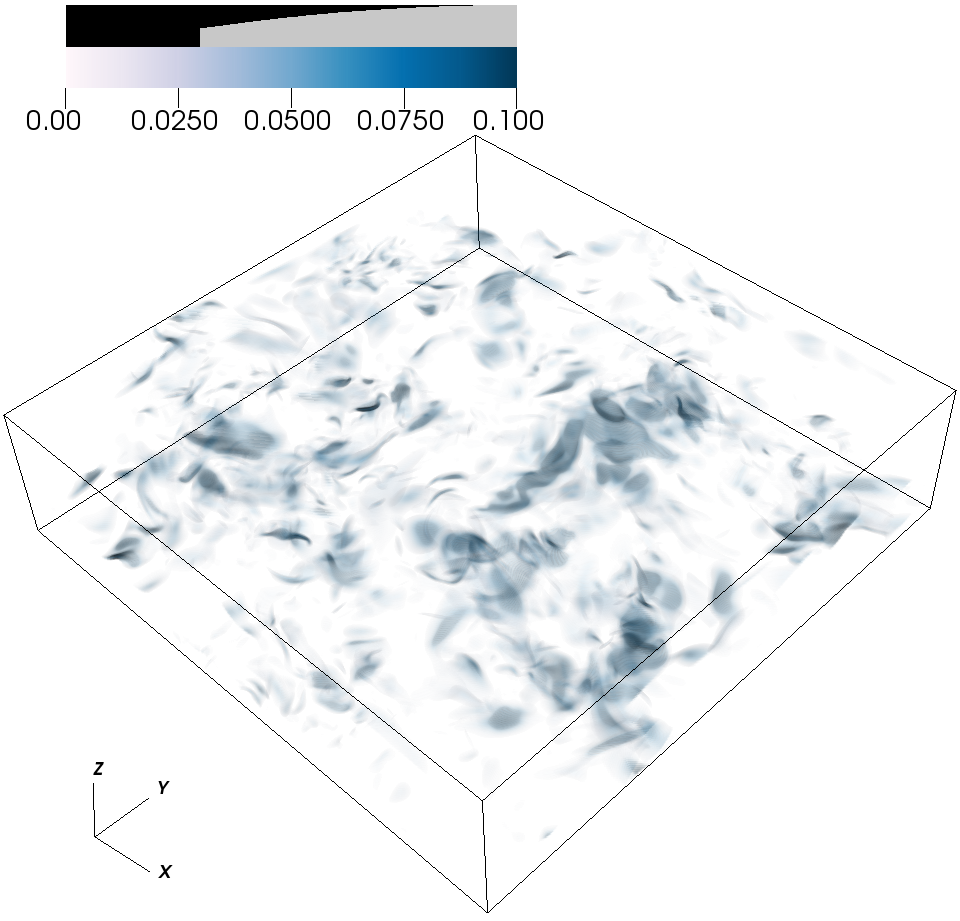
\includegraphics[width=.95\textwidth]{files/chi_Om0.5_vr2.png}
    \emp
     \bmp{.31}
        %omega_z
        \centering
        $1/Ro = 2$
        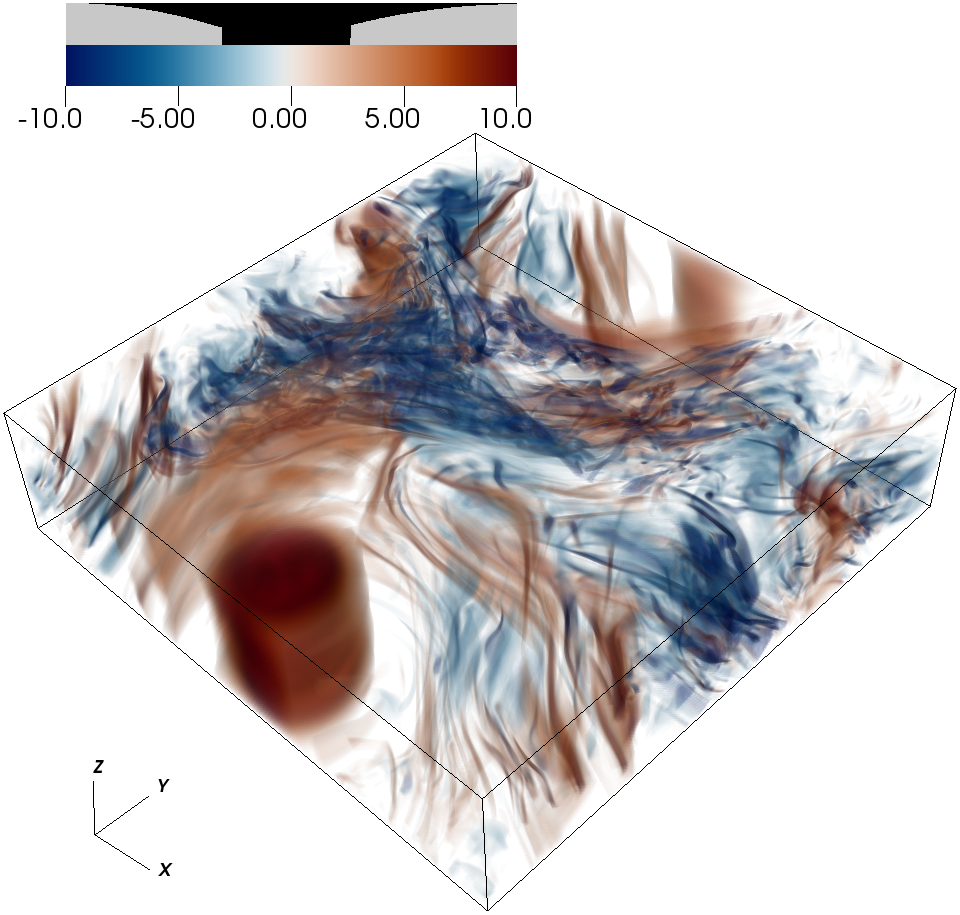
\includegraphics[width=.95\textwidth]{files/vortz_Om2_vr2.png}
        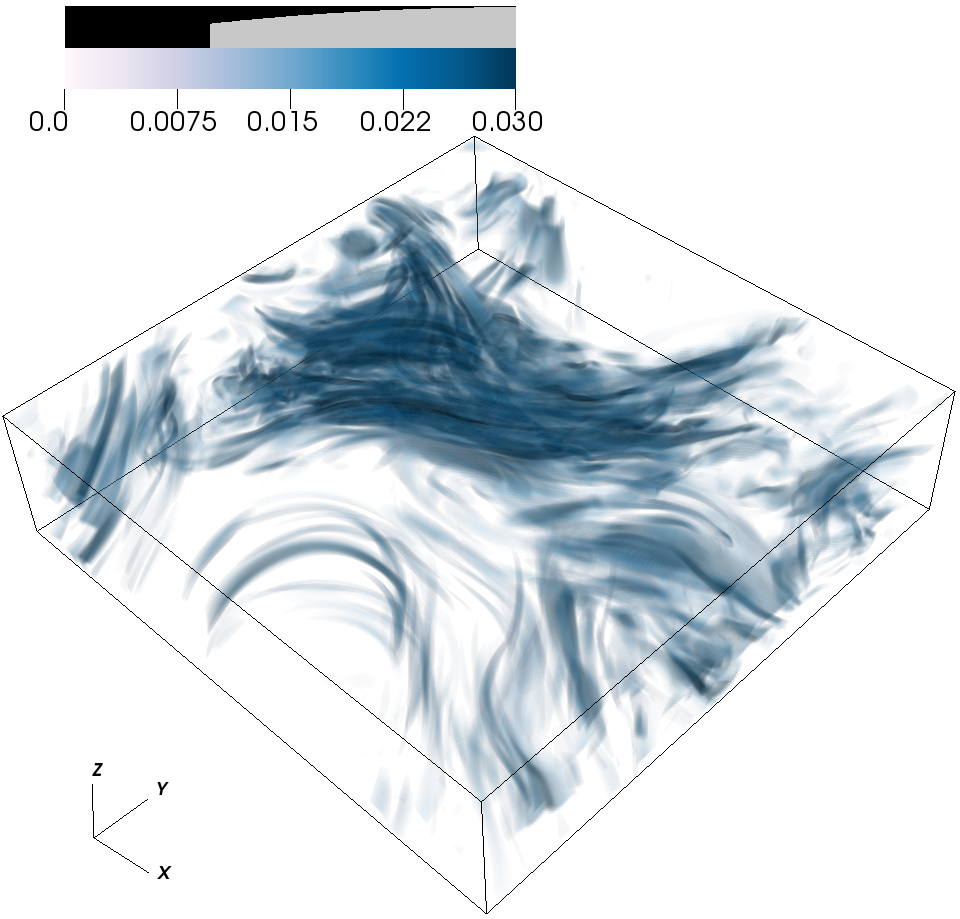
\includegraphics[width=.95\textwidth]{files/chi_Om2_vr2.png}
    \emp
    \bmp{.31}
        %omega_z
        \centering
        $1/Ro = 10$
        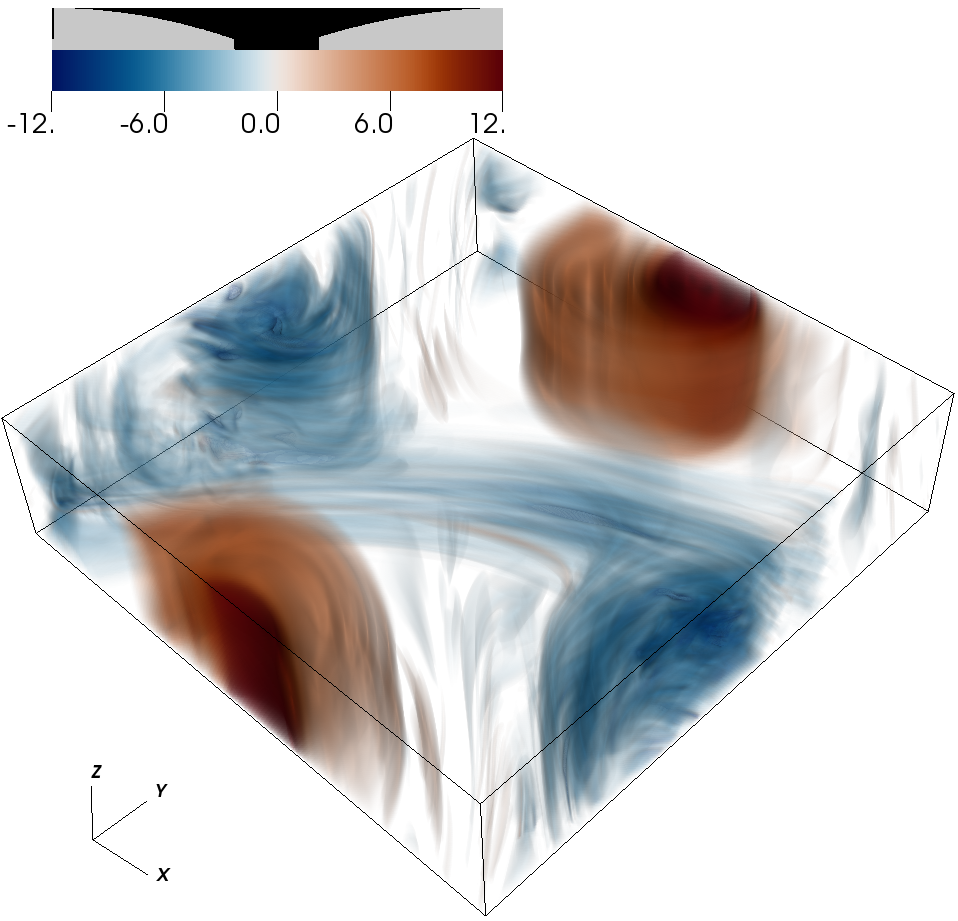
\includegraphics[width=.95\textwidth]{files/vortz_Om10_vr2.png}
        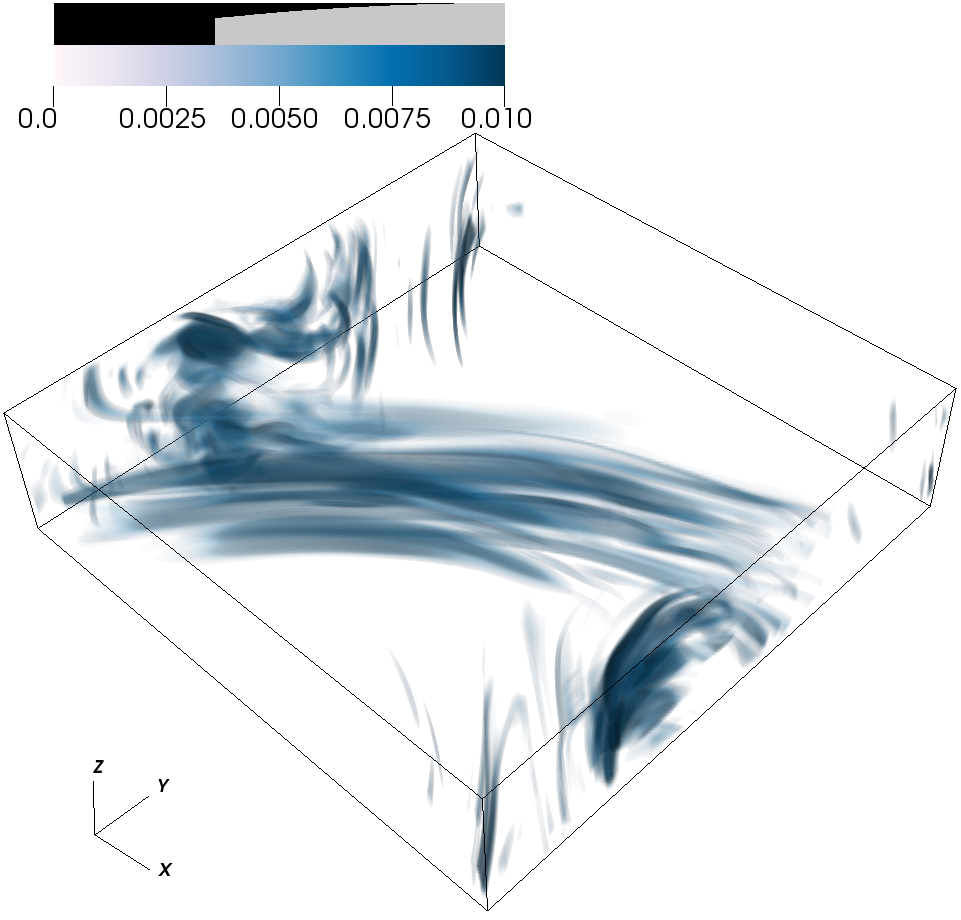
\includegraphics[width=.95\textwidth]{files/chi_Om10_vr2.png}
    \emp
\end{frame}

\begin{frame}{Quantities affected by Rotation}
    \bmp{.49}
        % u_h
        \centering
        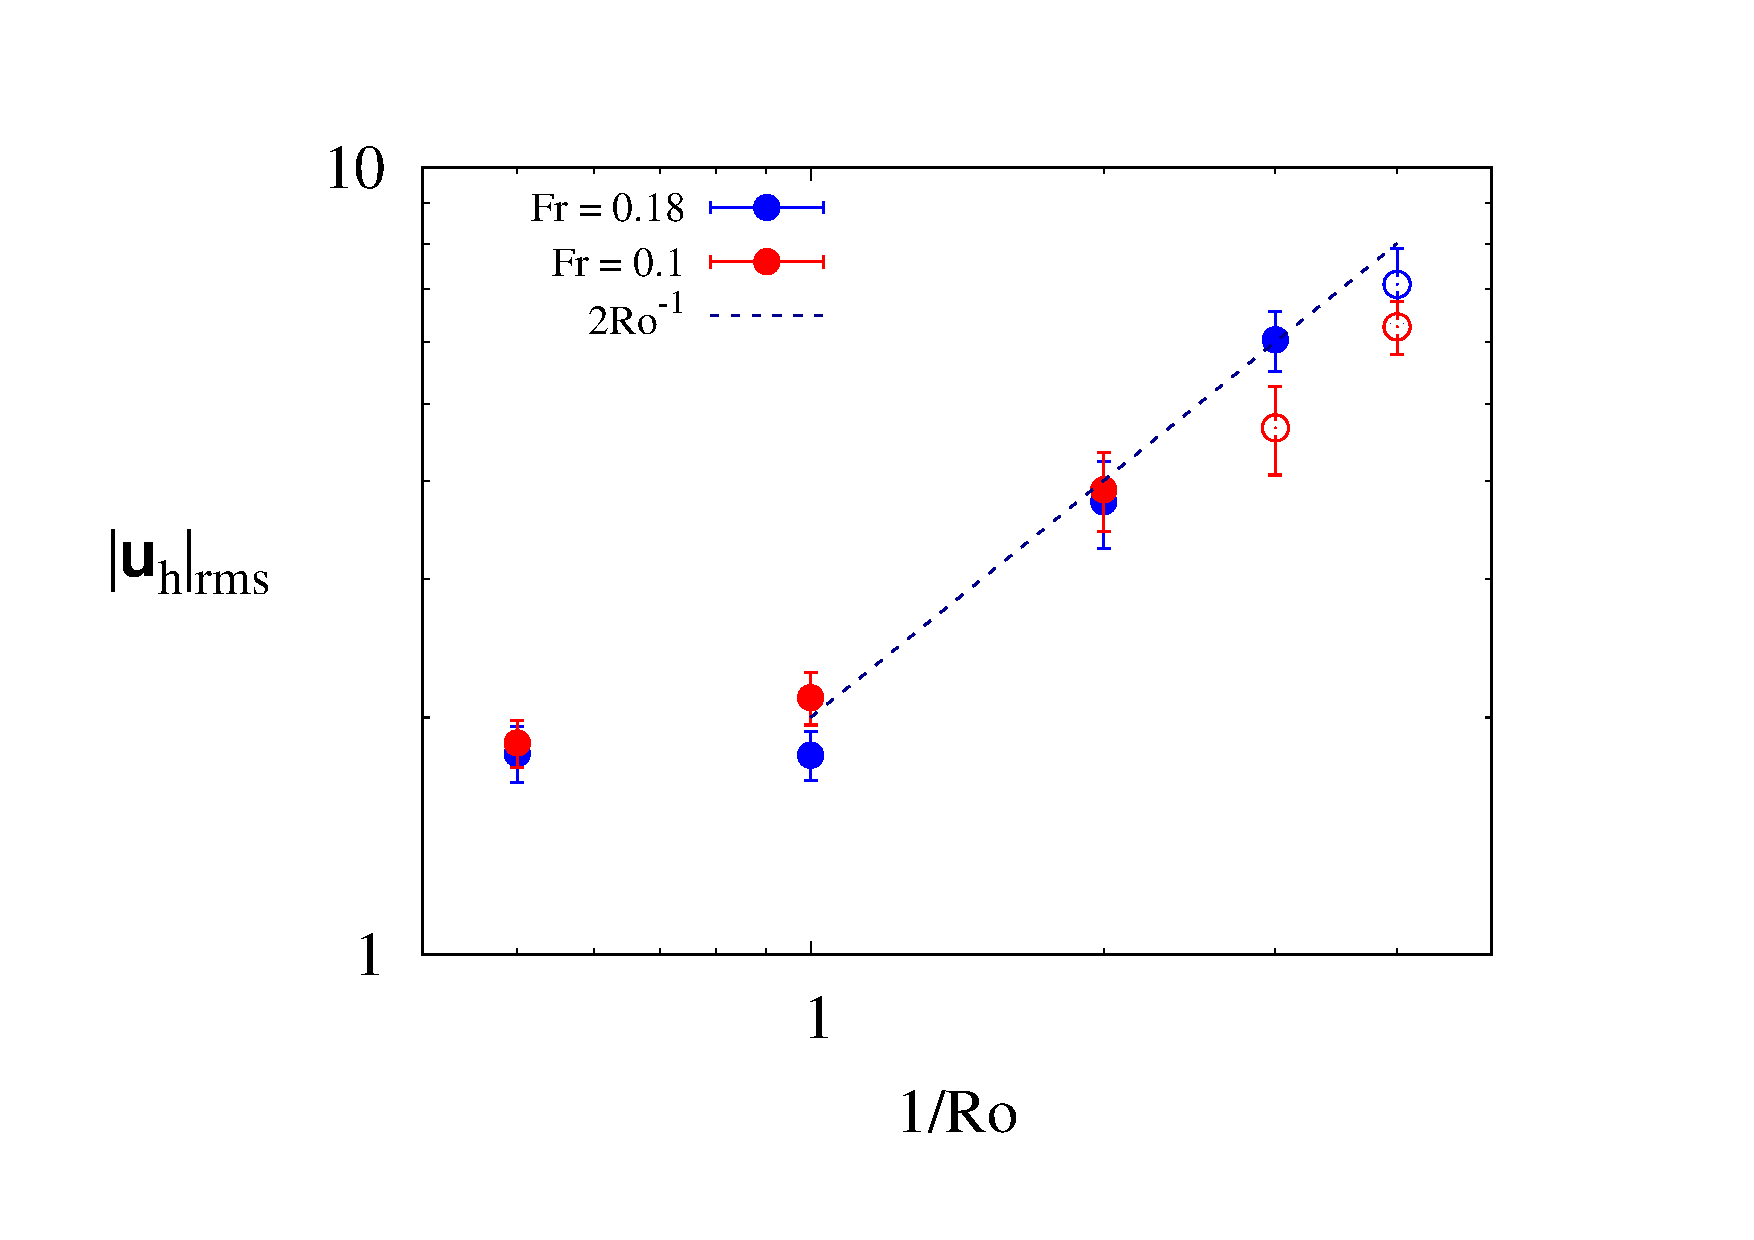
\includegraphics[width=.83\textwidth]{files/urms_plot.pdf}
    
         % mixing efficiency
        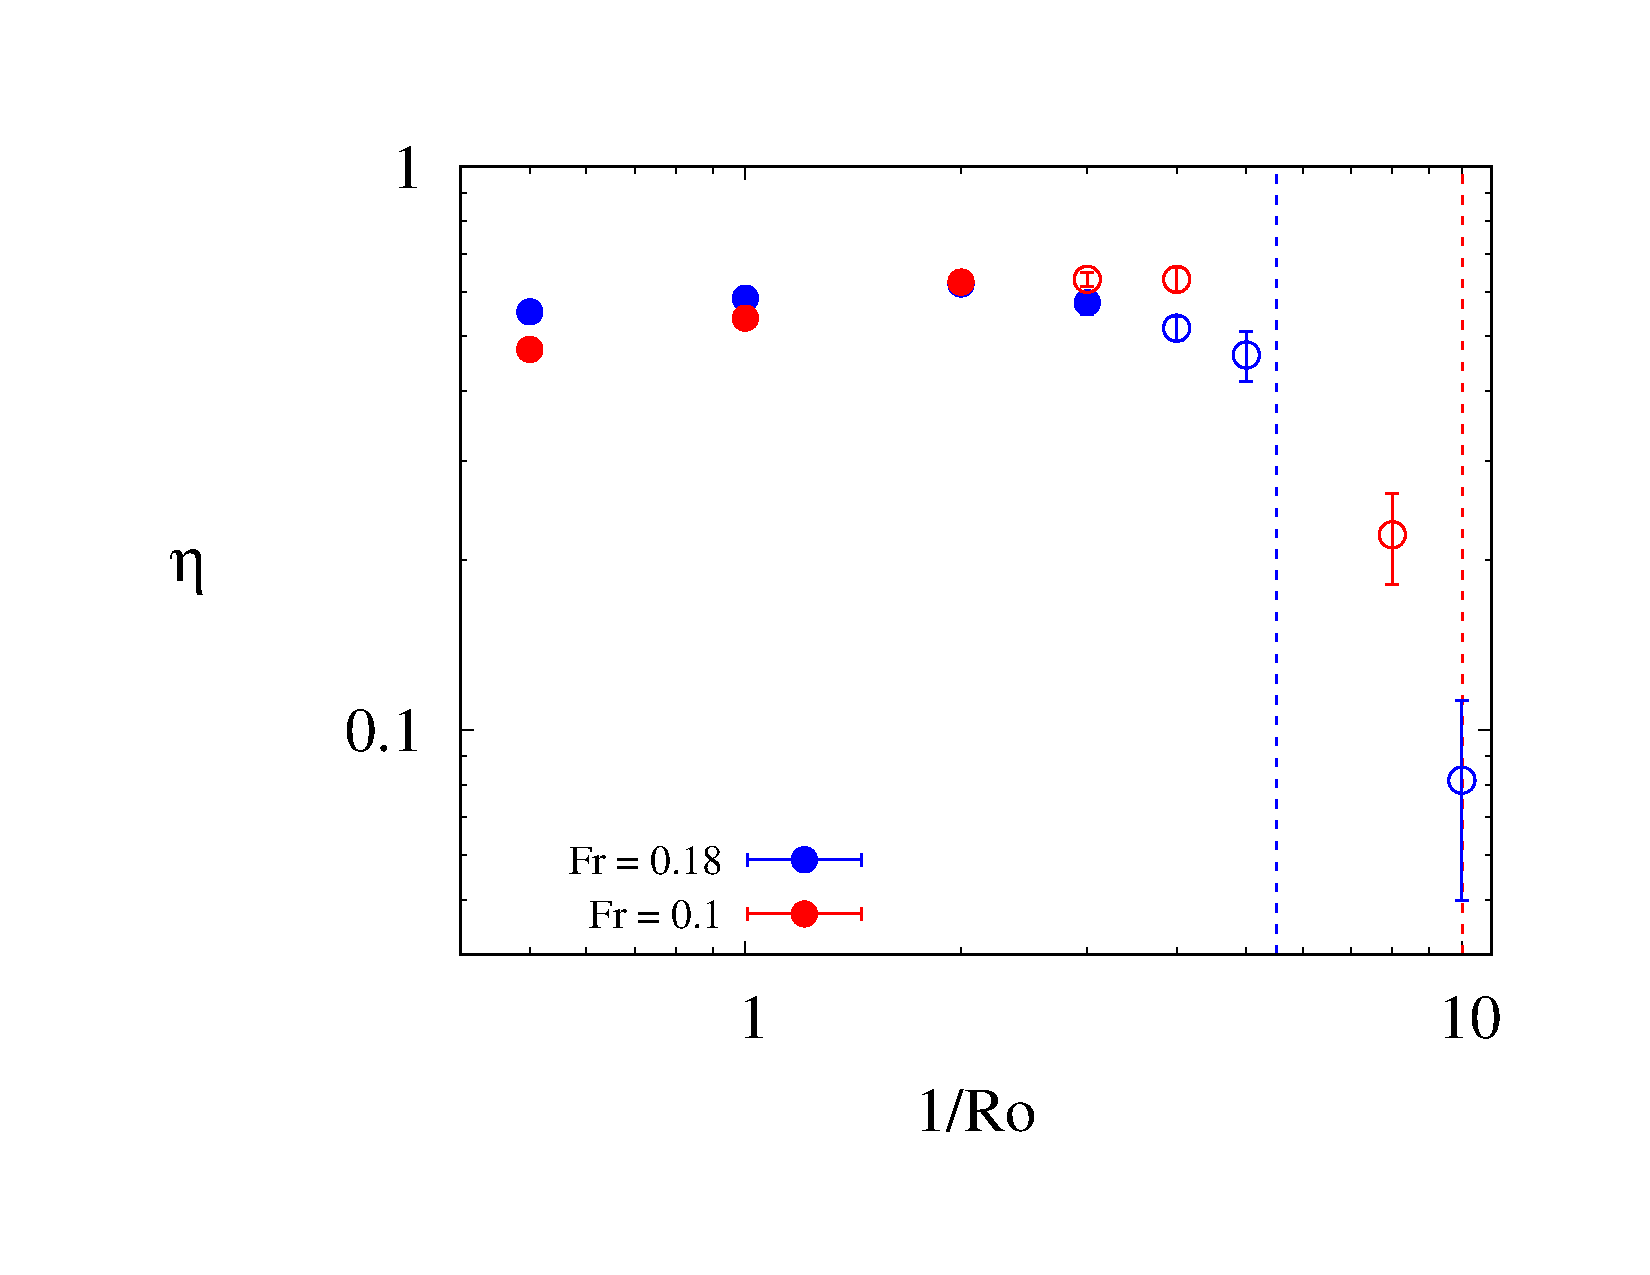
\includegraphics[width=.8\textwidth]{files/mixing_plot.pdf}
    \emp
    \hspace{2pt} 
    \bmp{.49}
         % temp flux efficieny
        \centering
        \includegraphics[width=.8\textwidth]{files/bflux_plot.pdf}

        % wrms plot
        \includegraphics[width=.8\textwidth]{files/wrms_plot.pdf}
    \emp
\end{frame}



\begin{frame}{Rotation in the Multiscale Theory}
    We now include the Coriolis term in the multiscale theory by \citet{Chinial2022} in order to study the effects of rotation on stratified turbulence.
\end{frame}

\begin{frame}{Weakly rotating regime: $Ro \ge 1$}

    \begin{itemize}
        \item Mean flow is weakly influenced by rotation.
        \item Fluctuations are not rotationally influenced.
    \end{itemize}
    {\scriptsize
    \begin{gather*}
    \ppts{\bar{\uvec}_h} + \bar{\uvec}_h\cdot \grads\bar{\uvec}_h
    + \frac{1}{\alpha}\overline{\uvec_h'\cdot\gradf\uvec_h'}
    + \frac{\bar{w}}{\alpha}\ppzeta{\bar{\uvec}_h} 
    + \overline{\frac{w'}{\alpha}\ppzeta{\uvec_h'}} + \frac{1}{Ro}\ez \times \bar{\uvec}\\
    = -\grads\bar{p} + \bar{\F}_h + \frac{1}{Re_b}\ppzetas{\bar{\uvec}_h} \tag{mean}\\
    \frac{1}{\alpha}\pptf{\uvec_h'} 
    + \frac{1}{\alpha}\bar{\uvec_h}\cdot\gradf\uvec_h'
    + \frac{w'}{\alpha}\ppzeta{\bar{\uvec}_h} + \frac{1}{Ro}\ez \times \uvec'\\
    = -\frac{1}{\alpha}\gradf p' + \frac{1}{Re_b}\left( \gradf^2\uvec_h' + \ppzetas{\uvec_h'}\right) \tag{fluctuations}
    \end{gather*}
    }
    No change in the scalings obtained by \citet{Chinial2022}.
\end{frame}

\begin{frame}{Intermediate regime: $\alpha \ll Ro \ll 1$}

    \begin{itemize}
        \item Mean flow is strongly influenced by rotation.
        \item Fluctuations are not influenced by rotation directly. 
    \end{itemize}
    {\footnotesize
    \begin{gather*}
        \frac{1}{Ro}\ez \times \bar{\uvec}_h = -\grad_s \bar{p}, \quad \ppzeta{\bar{p}} = 0 \tag{mean}
    \end{gather*} 
    \begin{equation*}
        \begin{split}
        &\frac{1}{\alpha}\pptf{\uvec_h'} 
        + \frac{1}{\alpha}\bar{\uvec}_h\cdot\gradf\uvec_h'
        + \frac{w'}{\alpha}\ppzeta{\bar{\uvec}_h} + \frac{1}{Ro}\ez \times \uvec'_h\\ 
        &= -\frac{1}{\alpha}\gradf p' + \frac{1}{Re_b}\left( \gradf^2\uvec_h' + \ppzetas{\uvec_h'}\right) 
        \end{split}
        \tag{fluctuations}
    \end{equation*}
    }
    
    \begin{itemize}
    
    \item Hydrostatic equilibrium in the fluctuation equations implies $\alpha = Fr$. 
\end{itemize}
\end{frame}

\begin{frame}{Strongly rotating: $Ro \ll \alpha$}

    \begin{itemize}
        \item Both mean flow and fluctuations are strongly rotationally influenced.
    \end{itemize}

    \begin{align*}
        \frac{1}{Ro}\ez \times \bar{\uvec}_h &= -\grad_s \bar{p}, \quad \ppzeta{\bar{p}} = 0 \tag{mean}\\
        \frac{\alpha}{Ro}\ez \times \uvec'_h &= -\grad_f p', \quad \ppzeta{p'} = 0 \tag{fluctuations}
    \end{align*} 

    What is $\alpha$?
\end{frame}

\begin{frame}{Missing Vertical Length Scale}
    The appearance of strong columnar vortices in the flow suggests that another vertical length scale is needed in order to create a multiscale theory of rotating stratified turbulence \citep[cf.][]{SpragueJulienKnoblochWerne2006, JulienKnobloch2007}.
    
\end{frame}

\begin{frame}{Conclusion}

    \begin{itemize}
        \item Stochastic forcing produces flow with notably different properties compared to steady forcing.
        \item Method of isolating mean and fluctuation dynamics must be modified.
        \item Rapid rotation influences the mean flow before it influences the fluctuations. Vertical mixing is only affected when $Ro \to Fr$
        \item In rapidly rotating flows, mixing is contained in regions of anti-cyclones.
        \item Very rapid rotation inhibits vertical mixing completely.
    \end{itemize}

\end{frame}

\begin{frame}{Future Work}
    \begin{itemize}
        \item Additional DNS to extend investigated parameter space ($Fr, Ro, Re, \ldots$).
        \item Comprehensive comparison of Steady vs. Stochastic forcing is necessary.
        \item Develop a multiscale theory of rotating stratified turbulence accounting for multiple vertical length scales.
    \end{itemize}
\end{frame}

{\scriptsize
\bibliographystyle{apj}
\bibliography{BuhlThesis}
}
\end{document}
